\documentclass[master,openright,twoside,color]{buaathesis}
\usepackage{booktabs}
\usepackage{graphicx}
\usepackage[ruled]{algorithm2e} % For algorithms
\renewcommand{\algorithmcfname}{算法}
\SetKwInput{KwData}{输入}
\SetKwInput{KwResult}{输出}

\begin{document}

% 用户信息
% !Mode:: "TeX:UTF-8"

% 学院中英文名,中文不需要“学院”二字
% 院系英文名可从以下导航页面进入各个学院的主页查看
% http://www.buaa.edu.cn/xyykc/index.htm
\school
{计算机}{School of Computer Science \& Engineering}

% 专业中英文名
\major
{计算机应用技术}{Computer Science and Technology}

% 论文中英文标题
\thesistitle
{基于神经网络的高性能语言建模技术研究}
{}
{Nerual Network Based Highly Efficient Language Modeling}
{}

% 作者中英文名
\thesisauthor
{姜楠}{Jiang Nan}

% 导师中英文名
\teacher
{荣文戈}{Rong Wenge}
% 副导师中英文名
% 注:慎用‘副导师’,见北航研究生毕业论文规范
%\subteacher{副导师}{subteacher}

% 中图分类号,可在 http://www.ztflh.com/ 查询
\category{TP391}

% 本科生为毕设开始时间;研究生为学习开始时间
\thesisbegin{2015}{09}{01}

% 本科生为毕设结束时间;研究生为学习结束时间
\thesisend{2018}{}{}

% 毕设答辩时间
\defense{2018}{}{}

% 中文摘要关键字
\ckeyword{层次概率,神经语言模型,递归神经网络,自然语言处理}

% 英文摘要关键字
\ekeyword{Hierarchical Softmax, Neural Language Model, Recurrent Neural Network, Natural Language Processing.}
% !Mode:: "TeX:UTF-8"

% 研究方向
\direction{自然语言处理}

% 导师职称中英文
\teacherdegree{副教授}{Associate Prof.}
% 副导师职称中英文
% 注:慎用‘副导师’,见北航研究生毕业论文规范
%\subteacherdegree{讲师}{Teacher}

% 保密等级,注:非保密论文时不需要此项
%保密论文请更改‘buaathesis.cls’里相应代码
%\mibao{机密}

%申请学位级别
\applydegree{工学硕士}

% 论文编号,由10006+学号组成
\thesisID{10006SY1506330}

% 论文提交时间
\commit{2018}{}

% 学位授予日期
\award{2018}{}{}


% 中英封面、提名页、授权书
%\maketitle
% 前言页眉页脚样式
\pagestyle{frontmatter}
% 摘要
\begin{cabstract}
最近在自然语言处理中,已经提出了基于神经网络结构的变体,并成功地应用于神经语言模型和神经声学模型。这些神经模型可以通过学习来自大规模语料库的参数来利用知识,而对于真实世界的挑战来说,它们是非常缓慢的,因为它们在训练和推理期间预测来自大词汇量的候选者。作为基于抽样的近似的替代,我们探索历史提出的基于树和基于类的分层softmax方法。在这项研究中,为了减少计算时间,并使其与现代图形处理单元兼容,我们引入了一系列高效和有效的方法,并将我们的贡献归类为:a)首先,我们改进它们的结构组成并引入一个紧凑的基于树和基于类的相应的分层softmax方法的损失函数; b)其次,我们讨论几种基于ngram的句法和语义聚类算法对各种类型层级softmax的影响,因为它们对聚类方法敏感; c)第三,我们讨论了可能的分层softmax变体的推理算法,保证模型可以在不同情况下获取可能的预测结果。最后,我们用标准基准数据集,即WikiText-2,WikiText-103和十亿字数据集对语言建模任务进行了我们的实验。与其他传统的优化方法相比,还实现了几个内在的评估指标的提升:单词错误率和困惑度。
\end{cabstract}

\begin{eabstract}
Recently in natural language processing, variants of neural networks based architecture have been proposed, and successfully applied to neural language models and neural acoustic models. These neural models can leverage knowledge by learning parameters from massive corpora, while they are extremely slow for the real world challenge as they predict candidates from a large vocabulary during training and inference. As an alternative to sampling-based approximation, we explore the historical proposed tree-based and class-based hierarchical softmax methods. In this research, aiming at reducing its computational time as well as making them compatible with modern graphics processing units, we introduce a series of efficient and effective approaches and categorise our contributions as: a) Firstly, we reform their structural composition and introduce a compact tree-based and class-based loss function for the corresponding hierarchical softmax methods; b) Secondly, we discuss the impact of several ngram-based, syntactic and semantic clustering algorithms for the vanilla hierarchical softmax as they are sensitive to clustering methods; c) Thirdly, we discuss possible inference algorithms for the hierarchical softmax variants, assuring the model can fetch presumable predictions under different circumstances. Finally, Our experiments were carried out on language modelling tasks with standard benchmarks datasets, i.e., WikiText-2, WikiText-103 and One Billion Word datasets. Consist improvement with several intrinsic evaluation criterions: word error rate and perplexity, were also achieved over other conventional optimisation methods.
\end{eabstract}
% 目录、插图目录、表格目录
%\tableofcontents
%\listoffigures
%\listoftables
% 符号表
%\include{data/master/denotation}

% 正文页码样式
\mainmatter
% 正文页眉页脚样式
\pagestyle{mainmatter}

\chapter{绪论}
\section{课题来源与意义}
近几年来,随着互联网(Internet)的兴起和发展,互联网上积累的数据呈现急剧膨胀的态势。根据国际数据信息公司\footnote{https://www.idc.com/}(International Data Corporation, IDC)的统计和预测,2018~年全球网络数据量已经达到~1.8~ZB,预计到~2025~年,全球网站数据累积总量还将增长约~50~倍。
随着这类文本、视频、图像无标注的数据(Unlabeled Data)的大量涌现,如何利用现有的机器学习算法(Machine Learning),从这类已存在的大量的无标注数据中学习内在规律和知识以提取出有用的信息,已经变成了一个重要的挑战\upcite{王建翔2017面向可读性评估的词向量技术研究及实现}。
自从2006 年,以~Geoffrey Hinton~为代表的学者们提出的深度学习(Deep Learning, DL)理念~\upcite{hinton2006reducing}以来,这一新的思路为解决如何利用爆炸的数据量,以提取有效知识带来了新的前景。
在这之后的发展中,基于神经网络(Neural Network,NN)的表示学习技术(Representation Learning)开始快速拓展到各个相关研究领域中去。
尤其在图像分类(Image Classification)、语音自动识别(Automatic Speech Recognition,ASR)~\upcite{DBLP:journals/taslp/WangW16}和神经机器翻译(Neural Machine Translation,NMT)~\upcite{bahdanau2014neural}领域的多个任务上,基于深度模型的方法,在精确度和效率上远远超过了基于特征提取(Feature Extraction)的传统方法。

随着应用领域的拓展,深度学习技术逐渐在自然语言处理中(Natural Language Processing, NLP)得到广泛应用。 例如,蒙特利尔大学教授 Yousha Bengio 提出用神经网络来训练语言模型(Language Model,LM),并对模型中的各个结构细节进行了相关探索\upcite{DBLP:conf/nips/BengioDV00}。因为输入的维度是固定的N个单词的词向量,而不是动态长度,所以该方法不能有效处理单词的长距离单词依赖问题。
针对这个问题,在后续的工作中,由其学生~Tomas Mikolov~提出了采用循环神经网络(Recurrent Neural Network, RNN)\upcite{DBLP:journals/cogsci/Elman90}对上下文信息作为建模策略的方法,并逐步将该理论进行了拓展和简化\upcite{DBLP:conf/interspeech/MikolovKBCK10}。
循环神经网络主要特点是能够记忆该单词之前的所有出现过的单词的信息,即所谓的全局上下文信息(Global Context),用来预测下一个单词出现的对数概率分布。
因为RNN模型在训练过程中学习到了单词的前面出现的所有词,所以句子的长距离依赖关系(Long Term Dependency)可以被学习到,所以该方法在建模理论上克服了最初的神经网络语言模型的无法利用语句长距离上下文依赖的缺点。
另外,在模型训练的过程中,语义相似的单词被映射到的某低维子空间中,也满足了单词的语义相似(Semantic Similarity)的要求。相比统计语言模型(Statistical Language Model)领域中的N-gram模型,他不需要平滑技术(Smoothing Technology)来对文本中出现次数少的单词做处理。
到目前为止,RNN~模型已经演变出各种结构,应用在非常多的文本任务上面,并且都能取得了较为满意的结果。

由于RNN网络的计算时间与句子的平均长度正相关,所以基于~RNN~建模的算法计算时间都很大,需要更长的时间收敛。同时,我们需要看到最简单的RNN模型所使用的参数数量是NPLM模型的两倍多,这也意味着RNN模型需要占用更大的内存空间,消耗了更多的计算资源,导致其无法广泛应用到现实场景中去。
在文献~\cite{DBLP:conf/icassp/MikolovKBCK11}~中,Tomas Mikolov 提出了多种优化策略来消除该模型的各种缺点,例如:缩短模型求导步数、对词表(Vocabulary)做分解~\upcite{DBLP:journals/coling/BrownPdLM92}等策略,这些计算策略能保证模型的计算精度,同时极大提高了RNN网络的运算效率。

\section{国内外研究现状}
语言模型可以用来估算一段文序列组合的可能性,该模型在机器翻译(Machine Translation)、语音识别(Speech Recognition)等任务上都有着极为重要的作用。考虑到语言模型的漫长的发展历史,我们可以划分为两个主要阶段:统计语言模型(Statistical Language Model)和神经网络语言模型(Neural Language Model)。
其中,统计模型指代的是~N-gram~语言模型,而随着深度学习的爆发,各种神经网络语言模型变体逐渐发展并占据了主导地位。我们接下来会对这两个演化阶段所涉及的算法一一介绍。

\subsection{N-gram 语言模型}
首先介绍传统的~N-gram~语言模型,该算法属于典型的基于稀疏表示(Sparse Representation)的语言模型,因为一个单词表示方式是独热表示(One-Hot Representation)。该传统模型的意义不仅是提供了一种文本建模策略,而且定义了如何评价语言模型的好坏,并且定义了语言模型所涉及的相关拓展方向。

接下来给出~N-gram~统计语言模型的形式化定义。假设给定一个长度为$m$ 的单词字符串,$w_1$ 到$w_m$ 依次表示这段文本中的各个单词,我们需要求解一个概率分布$p(w_1,\cdots,w_m)$,以表示该字符串存在或者出现的可能性。在求解过程中,我们通常使用链式法则(Chain Rules),将计算整个序列概率问题分解成如下形式:
\begin{equation}
\setlength{\abovedisplayskip}{6pt}
\setlength{\belowdisplayskip}{6pt}
\label{equ:lm}
p(w_1,\cdots,w_m) =p(w_1)\prod_{t=1}^{m}p(w_t|w_1,\cdots,w_{t-1})
\end{equation}
在实际求解过程中,如果文本的长度较长,公式~(\ref{equ:lm})~中右部~$p(w_m | w_1,w_2,\cdots,w_{m-1}) $ 的估计误差会很大。因此,提出了~N~元模型(N-gram model),它能简化了实际问题的复杂度,最早被用来估算条件概率。需要注意的是,单词距离大于$n$单词会被直接忽略,该模型可以写成如下形式:
\begin{equation}
\setlength{\abovedisplayskip}{6pt}
\setlength{\belowdisplayskip}{6pt}
\label{equ:approx}
p(w_i | w_1,w_2,\cdots,w_{t-1})  \approx p(w_i | w_{t-(n-1)},\cdots,w_{t-1})
\end{equation}
假若~$n=1$~,此时称其为一元模型(Uni-gram model),公式~(\ref{equ:approx})~将会退化成~$p(w_i),i\in [1,n-1]$.此时,整个句子的概率计算公式为:~$p(w_1,w_2,\cdots,w_m) = p(w_1)p(w_2) \cdots p(w_m)$。
从这个退化的公式中,可以得知:在一元模型中,整个文本的概率是出现的各个单词的词频概率的乘积,它直接丢失了文本词组之间的顺序信息。当~$n = 2$~时,称为二元模型(Bi-gram model),公式~(\ref{equ:approx})~将会退化为 $p(w_t|w_{t-1})$。除此之外,还有 $n=3$ 时的三元模型(Tri-gram model),使用$p(w_t |w_{t-2},w_{t-1})$ 作为近似概率分布。当~$n>1$~的模型均可以保留一定的词序信息。

传统方法采用单词或者n元组的词频来作为n元组的概率计算方法,该方法简单有效能满足线上负载的计算需求。但是随着n的增大,模型的参数呈现指数爆炸式增长、概率计算复杂度也相应上升。目前谷歌有在线存储的最大的~9~元模型(Google N-gram Viewer)\footnote{https://books.google.com/ngrams},这已经是目前计算机系统存储,数据访问的极限了。


神经网络的建模思路源自于~N-gram~模型,它主要解决的问题是如何对文本的上下文信息利用先用的模型进行建模。历史上的模型,我们可以主要划分为:传统前向传递神经网络(Feed Forward Neural Network, FFNN)、循环神经网络(Recurrent Neural Network, RNN)以及双线性模型(Bilinear Model)这三种建模方案。 以下我们将一一探讨。


\subsection{前馈神经网络语言模型}
由于神经网络对参数进行高度共享,因此对低频词具有天然的平滑能力。这里所指的神经网络语言模型(Neural Probabilistic Language Model, NPLM) ,最早由Bengio等人在2001年提出\upcite{DBLP:conf/nips/BengioDV00}, 近年来一些学者开始展开这方面的研究,并取得一系列成果,如~\cite{DBLP:conf/acl/BaroniDK14,DBLP:journals/sigkdd/BellK07,DBLP:journals/pami/BengioCV13,DBLP:journals/tnn/BengioSF94}~。 但总体而言, 对NPLM的研究还处在起步阶段。具体而言,NPLM通过一个多层感知网络(Multi-Layer Perceptron, MLP)来计算公式~(\ref{equ:approx})~中概率。
\begin{figure}
  \centering
  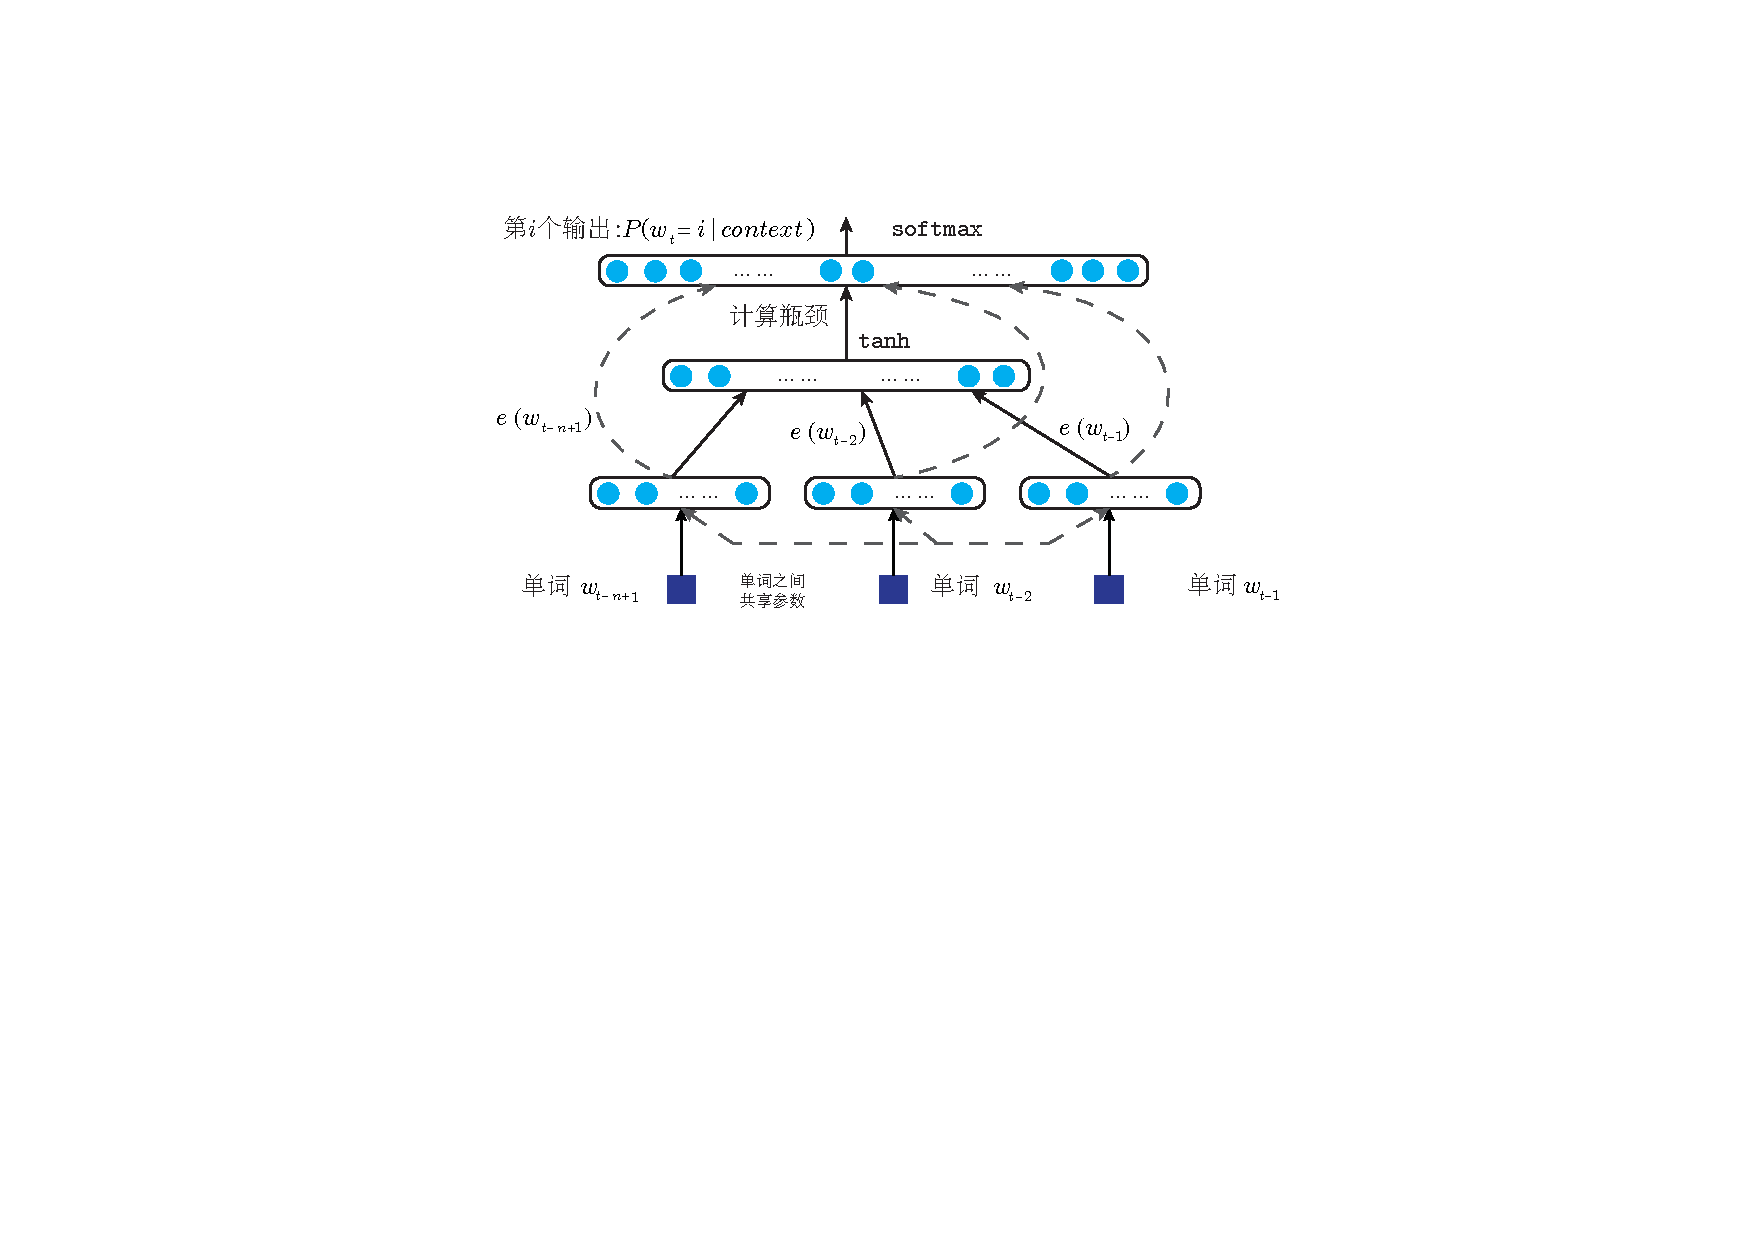
\includegraphics[width=.85\linewidth]{./figures/nplm.pdf}
  \caption{前馈神经网络语言模型}\label{fig:nplm}
\end{figure}

图~\ref{fig:nplm} 给出一个典型的采用三层前馈神经网络结构 NPLM 语言模型。其中输入层用于表征前$n$个单词的高维分布;隐藏层,表征单词的上下文信息,最后一层是输出预测层,预测下一时刻的可能出现的单词概率分布。为了解决数据稀疏问题,Bengio~等人提出拼接(Concatenation)各词的词向量作为输入,如下所示:
\begin{equation}\label{equ:we}
  x = [e(w_{i-(n-1)}), \cdots , e(w_{i-2}), e{(w_{i-1})}]
\end{equation}
模型的隐藏层$h$ 和输出层$y$可以依照下面的公式计算获得:
\begin{equation}\label{equ:nplm}
\setlength{\abovedisplayskip}{6pt}
\setlength{\belowdisplayskip}{6pt}
\begin{split}
h =& \tanh(Hx+b) \\
y =&Wx + Uh +b'
\end{split}
\end{equation}
其中参数矩阵~$H,W,U$~指代层与层之间的权重\upcite{赵林2007一种新的基于结构的神经网络规则抽取方法},参数向量~$b,b'$~均为模型中的偏置项(Bias)。如果存在$W$,那么模型能直接学习一个线性模型,需要训练的时间减少;如果不存在$W$,模型学习到非线性的网络模型,具有更好的泛化性(Generalization)。因此在后续工作中,很少有使用输入层到输出层直连边的工作,下文我们也直接忽略这一种直连的操作。假设不考虑$W$ 矩阵,整个模型计算量最大的运算,就是从隐藏层到输出层的矩阵运算$Uh$,后续的模型均有对这一矩阵乘法计算做优化。

\subsection{对数双线性语言模型}
2007 年,Mnih 和 Hinton 在神经网络语言模型(NNLM)的基础上提出了对数双线性语言模型(Log-Bilinear Language Model, LBL)~\upcite{DBLP:conf/icml/MnihH07}。LBL~模型与~NNLM~模型的区别正如它们的名字所示,其中~LBL~的模型结构是一个对数双线性结构;~NNLM~的结构不包含双线性结构,仅仅是简单的前馈网络。具体来讲,LBL 模型的代价函数为:
\begin{equation}
\setlength{\abovedisplayskip}{6pt}
\setlength{\belowdisplayskip}{6pt}
\label{equ:lbl}
\begin{split}
   &\hat r=\sum_{i=1}^{n-1}{U_i e({w_i})}, \\
   &p(w_n=w|w_{1:n-1})=\frac{\exp(\hat r^\top e(w))}{\sum_j{\exp(\hat r^\top e(w_j))}}
\end{split}
\end{equation}
其中 $\hat r$ 代表了语言模型的上下文信息,$U_i$ 指代的是对应单词的权重向量。然后基于上下文信息表示 $\hat r$ 和下一个单词的目标词汇表中所有单词 $e(w),w\in \mathcal{V}$ 的表示之间的相似度来计算下一个单词的可能的概率分布。

公式~(\ref{equ:lbl})~所描述LBL模型的代价函数与公式~(\ref{equ:nplm})~所描述~NNLM~模型的代价函数的主要区别有:1) LBL 模型中,没有非线性的激活函数$\tanh$,而由于NNLM 是非线性的神经网络结构,激活函数必不可少;2) LBL 模型中,只有一份词向量$e$,也就是说,无论一个词是作为上下文,还是作为目标词,使用的是同一份词向量。其中第二点(只有一份词向量),只在原版的LBL 模型中存在,后续的改进工作均不包含这一特点。

后来,Mnih~等人以~LBL~模型为基础,并对其所存在缺点做了一系列改进工作。其中最重要的模型有两个:逆向量语言模型(inverse vector LBL,ivLBL)~\upcite{DBLP:conf/nips/MnihK13}和层次对数双线性语言模型(Hierarchical LBL,HLBL)~\upcite{DBLP:conf/icml/MnihT12}。

\subsection{循环神经网络语言模型}
对于循环神经网络来说,它能直接对序列概率~$p(w_t | w_1,w_2,\cdots,w_{t-1})$~进行建模,而不使用公式~(\ref{equ:approx})~对其进行简化~\upcite{mikolov2012statistical,DBLP:conf/interspeech/MikolovKBCK10} 。RNNLM 模型结构如图~\ref{fig:rnnlm}~所示,它的核心方法在于其隐藏层的计算公式:
\begin{equation}
\setlength{\abovedisplayskip}{6pt}
\setlength{\belowdisplayskip}{6pt}
\label{equ:rnn}
  h_t \leftarrow  \phi(e(w_t) + U h_{t-1} +b),
\end{equation}
其中 $\phi$ 为非线性激活函数。在上述公式中,$h_t$ 表示文本中第 $t$ 个词 $w_t$ 所对应的隐藏层,该隐藏层由词向量 $e(w_t)$ 以及上一个步的隐藏层输出 $h_{t -1}$ 计算得到。隐藏层的初始状态为$h_0$,随着模型逐个读入单词:$w_1,w_2,\cdots$, 隐藏层根据公式~(\ref{equ:rnn})~被计算出来并被输出:$h_1,h_2,\cdots$ 。通过这种自身迭代更新方式,囊括了此单词前所有上文的信息,相比NPLM模型,RNNLM 理论上能学习到更丰富、更长距离的知识,也有更大的潜力达到更好的效果。最后,RNNLM 模型的输出层与NPLM 模型的输出层都采用softmax算法,两者是一致的。

\begin{figure}
  \centering
  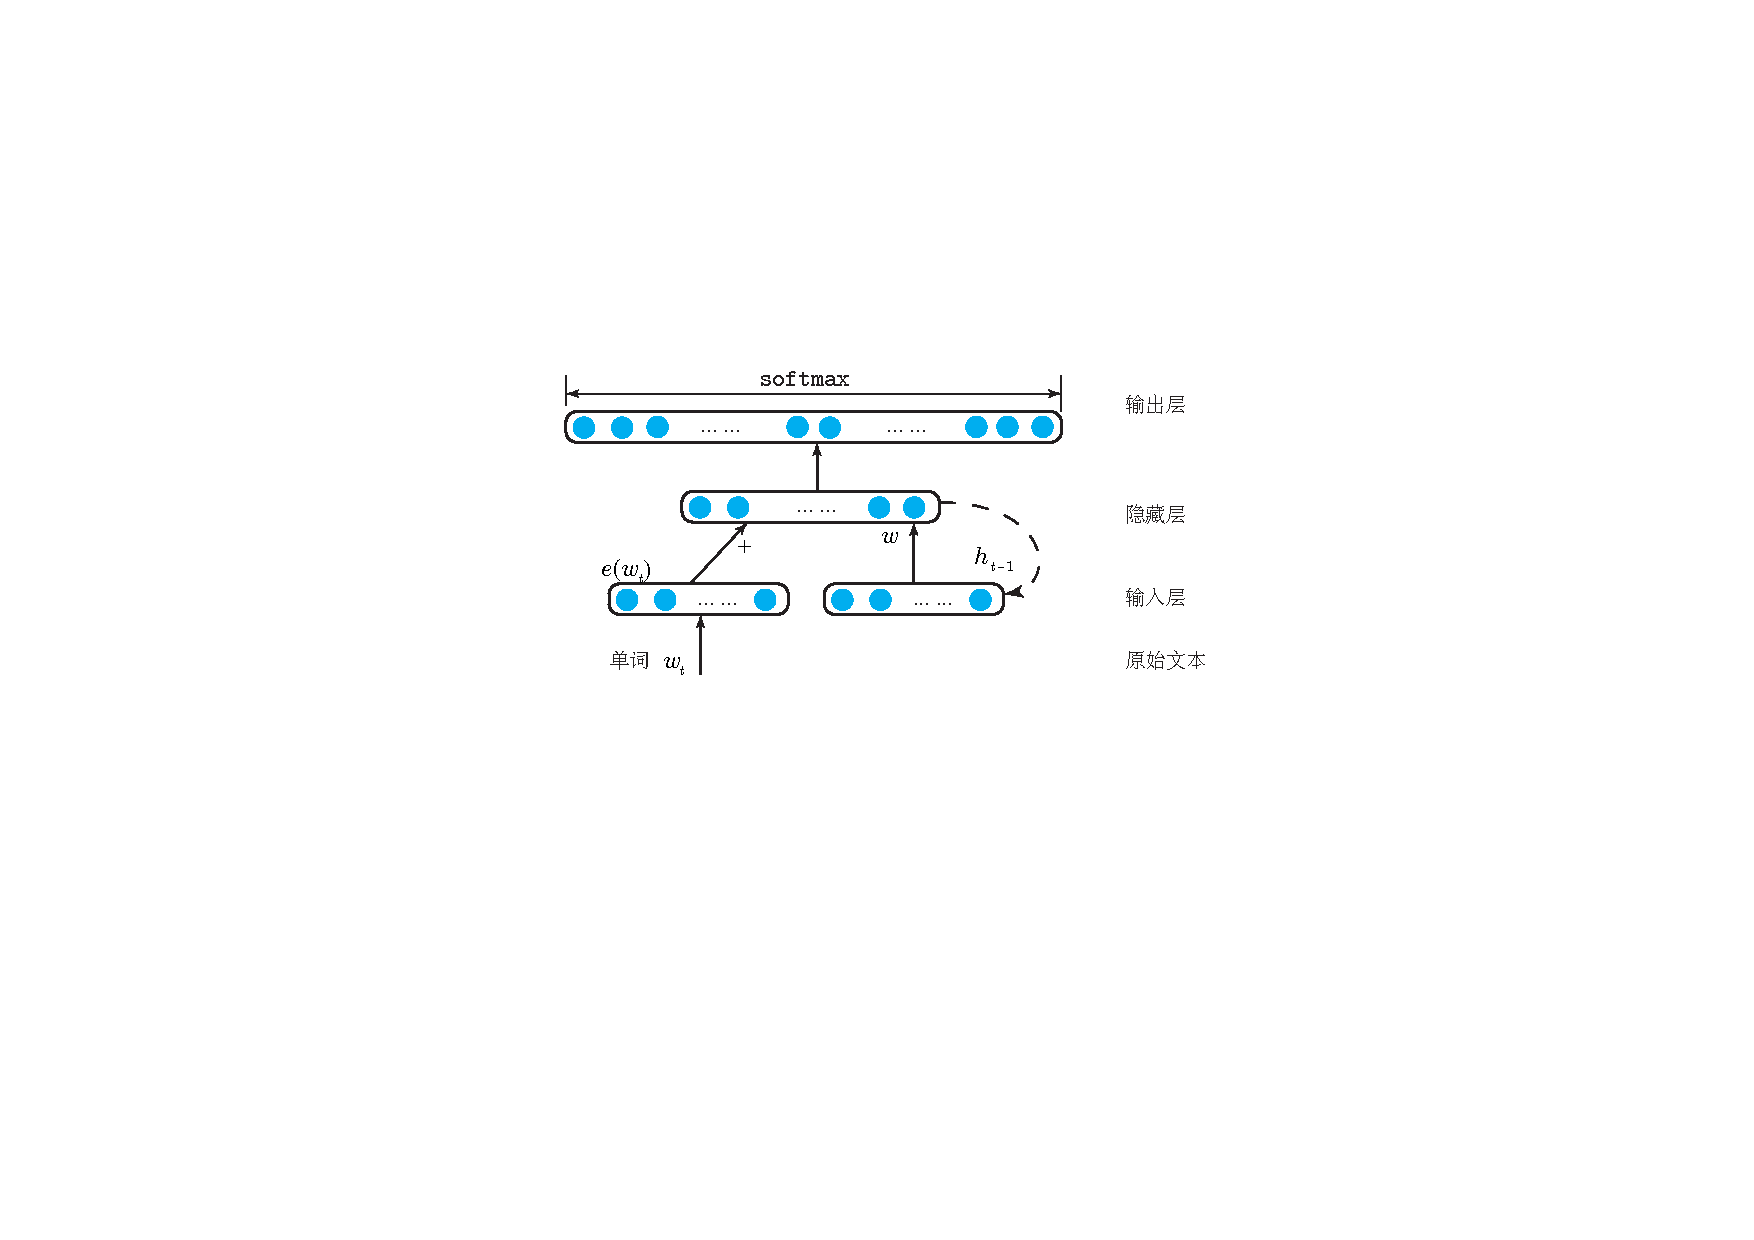
\includegraphics[width=.8\linewidth]{./figures/rnnlm.pdf}
  \caption{循环神经网络语言模型结构图}\label{fig:rnnlm}
\end{figure}


除了介绍的两种经典的建模方法,最近研究者提出可以使用带有门限机制(Gating)的RNN来防止模型的长距离依赖问题,例如长短记忆网络(Long Short-Term Memory, LSTM), 门限记忆节点(Gated Recurrent Unit, GRU)和其他网络。


\section{论文研究内容}
在历史文献当中,源词和目标词分别被称为模型的输入和输出。源词通常可以用分布式表示(Distributed Representation)来表示,称为输入词嵌入(Word Embedding),可以使用基于外部语料库的连续词袋模型(CBoW)或跳跃单词模型(Skipgram)模型来训练。而这两个模型来源于语言模型任务,并且为了在特征空间中产生可能的嵌入分布而被大大简化。另外,输出字通常表示为字索引(Indexing)或~$1-K$~编码,并且可以与softmax概率函数直接关联。

语言模型的大词表问题是目前理论应用到实际过程中必须要克服的问题,我们当然可以通过配置高性能服务器来暂时延缓该问题的后果。但是一旦应用到大数据集上,即使是目前最好的中央处理器(CPU)或者图形处理器通用计算(GPGPU),仍然需要一个多月时间才能训练完善。因此,在保证原有模型的准确率和精度的前提下,如何提高模型的训练速度是我们主要讨论和研究的内容。为此我们讨论了两个不同的内容:上下文信息建模效率和精度对比和大词表问题的优化和研究。

针对上下文信息建模手段,目前主要采用的方案有以下几种:一种是采用子词(Subword-level)或者字符级别的词(Character-level)来直接缩小词表大小;一种是通过采样技术(Sampling-based Approximation)来减少必要的训练时间;一种是通过基于分类的多元分类(class-based Hierarchical Softmax, cHSM)来加速模型和采用基于树模型的多层二元分类模型(tree-based Hierarchical Softmax, tHSM)。同时,我们还需要针对CPU 和GPGPU设备分别进行探讨。因为传统的线性运算模型在流行的GPGPU并行运算方案中并不适用,所有需要结合不同的运算设备分别讨论可行的方案。

在本节中,我们将这个目标词表示扩展到一个分层的形式,使它们适配基于类和基于树的分层概率计算。首先,我们提出了一个在分层结构上建模参数的字编码方案。因此,考虑到~GPGPU~上的并行吞吐性能,我们推导出紧凑的代价函数及其梯度。同时,类或树上的单词分布对其性能有很大的影响,应该在训练阶段之前定义,这些动态交换算法在训练过程中改变了单词群或子树结构在这个研究中。我们采用了几个分层聚类和词汇分割策略,用统计,句法和语义知识来初始化其结构,以达到一个稳定和可以预期的性能。而且,在推理过程中,不同于传统的softmax情况,得到最好的候选者自然是可行的,层次推理不能直接用 softmax 方法来实现。我们讨论基于树和基于类的搜索策略的两种不同的推理情况:1)打分:输出给定序列的概率;2)排序   :在给定的上下文中获取得分最高的一个候选单词。
\section{论文的组织结构}
\textbf{第一章:}``绪论'',主要介绍了本论文的研究背景和意义,另外简要说明了语言模型的发展历史以及本文的主要工作,并对本文的组织架构进行了说明。

\textbf{第二章:}``相关技术介绍'',对历史上的各个学术流派在语言模型的任务上相关工作进行了介绍。

\textbf{第三章:}``并行树状概率模型'',介绍了基于二叉树的层次概率模型,并比较了传统树状模型的差一点。同时还研究了在推理测试阶段,二叉树层次概率模型能应用的策略,以保证实际测试结果性能和效率。


\textbf{第四章:}``并行分类层次概率模型'',介绍基于分类的层次概率模型,并分析了词表非均匀划分所产生的后果,进而探讨了类别不均匀问题所带来的影响以及相关解决策略。最后探讨了在测试阶段,语言模型的任务需求和分类层次概率模型相应的解决算法。

\textbf{第五章:}``语言模型实验及实验结果分析'',实证研究了本论文提出的并行层次概率模型的实际效果,并和其他算法在各个指标维度上进行了比较和分析。

最后结论部分,总结了全论文的贡献和工作,并提出了未来的工作方向,同时撰写了结束语。




\chapter{相关技术介绍}
\section{引言}
在自然语言处理研究领域中,基于神经网络的分布式表示(Distributional Representation)一般统称为词向量(Word Vector)、词嵌入(Word Embedding)或者分布式表示(Distributed Representation)~\upcite{DBLP:conf/nips/MikolovSCCD13}。神经网络词向量表示技术,是通过神经网络技术对:1)单词的语境,即上下文(Context);2)以及上下文与下一步的目标单词之间的关系(Next-Utterance Prediction),这两个主要的部分进行建模。
由于神经网络结构或各种组合较为灵活,这类方法的最大优势在于可以表示复杂的上下文语义(Complex Context)。历史上的方法主要是基于单词共现矩阵(Co-occurrence Matrix)的分布表示方法,最常用的上下文仅仅是利用了单词的顺序信息。单词的语义向量是通过给这个单词共现矩阵进行矩阵分解,例如奇异值分解(Singular Value Decomposition,SVD),潜在语义分析(Latent Semantic Analysis,LSA),也可以写成潜在语义索引(Latent Semantic Indexing,LSI)分解算法。其中对于SVD分解算法,第一个分解获得的矩阵就是我们模型输出的单词的词向量矩阵。然而,如果使用包含词序信息的~N-gram~作为上下文,当~$N$~增加时,N-gram 的所需要存储的单词序列总数会呈指数级增长,此时会遇到维数灾难问题(Curse of Dimensionality)\footnote{https://en.wikipedia.org/wiki/Curse\_of\_dimensionality}。这一瓶颈深深限制了~N-gram~模型的实际应用。而用神经网络替代表示~N-gram~的单词概率分布时,可以通过一些组合方式对~N~个词进行组合,其优点显而易见:神经网络语言模型所需要的参数数量仅以线性速度增长。有了这一优势,神经网络模型可以对更复杂的上下文进行建模,在从训练后的模型提取出来的词向量中包含更丰富的语义信息。

到目前为止,在语言模型的研究领域中,所应用到的神经网络模型主要包括: 传统前向传递神经网络(Feed Forward Neural Network, FFNN)、循环神经网络(Recurrent Neural Network, RNN)三种基本的建模方案。当然基于这些基本组件,我们还可以构造更复杂的模型结构,但是我们无法保证复杂模型一定在效率和精确度上优于简洁的模型结构。复杂的模型可以表征更复杂的本文语义信息,例如句子的依存关系结构或者句子的句法分析树结构,但是这样的效果不一定能保证模型的泛化性能(Generalization)会很好,因为日常聊天文本的语序是混乱的,很难找到学者良好定义的句子关系,所以也无法让模型从混乱的文本分布中学习到有效的句子结构,以提升模型的精度。最好的模型,显然是假设越弱越合适,因为针对复杂的网络文本数据,我们模型训练所需要的要求越弱,模型越容易收敛并获得我们想要的结果。模型假设越强,模型所需要的数据质量越高,实际稳定性就会降低,产生得不偿失的后果。

语言模型的历史发展
除此以外,针对在本论文所讨论的语言模型的大规模应用过程中所遇到的大词表问题,目前现有的主要解决方法主要可以分为以下三种种策略:单词拆分算法(Vocabulary Truncation)、采样估计模型(Sampling-based Approximation)和层次分解模型(Vocabulary Factorisation),我们会在接下来的章节陆续介绍。其中本论文重点是研究基于类别的多元分类模型(class-based hierarchical softmax, cHSM)和基于二叉树的二元分类模型(class-based hierarchical softmax,tHSM),这两种算法我们分别在下一章更详细讨论和介绍。

\section{语言模型}
在这一节中,我们将首先从语言模型提出的实际任务的形式化定义开始,以阐述语言模型的训练目标和实际应用场景~\upcite{DBLP:journals/tnn/ChienK16}。一个好的语言模型应当考虑对文本的两种特征进行建模:语法特征(Syntactics)和语义特征(Semantics)。为了保证语法的正确性,我们往往只需要考虑生成的单词的前面的上下文(Previous Context),这也就意味着语法特性往往只对局部特征(Local Representation)进行建模。而语义特征的一致性则复杂了许多,它意味着我们需要考虑更大、更完善的上下文信息乃至整个文档语料,来获取正确的全局语义(Global Context)而不仅仅是局部语义信息(Local Context)。


具体地来说,给定一个包含$T$个单词的序列:$w_1,w_2,\cdots,w_T$,这个序列的对数概率(Log-probability),即描述该序列作为一个合理且合法的句子的流畅性(Fluency)概率和出现该单词组合的句子的可能性( Likelihood),可以使用马尔可夫链规则分解成一系列的条件概率的联合分布:
\begin{equation}
\label{laguage_model}
 \log p(w_1,\cdots, w_T ) = \sum_{t=1}^T \log p(w_t | w_{1:t-1}),
\end{equation}
其中前 $t-1$个单词在本论文中一律记作$w_ {1:t-1}$。进而,条件概率~$p(w_t | w_ {1:t-1})$表示给定其前面上下文$w_ {1:t-1} $作为预测的下一个单词的条件概率分布(Conditional Probability)。最早的传统方法可以由前馈网络来建模这个上下文信息, 同时用多标签概率函数(Multi-class Classification)来表示下一个单词的概率分布计算公式~\upcite{DBLP:journals/jmlr/BengioDVJ03}。 在训练的过程中,整个模型以最小化每个单位预测步骤里面的交叉熵损失(Cross Entropy Loss):
\begin{equation}\label{equ:losses}
  \ell=\sum_{t=1}^{T}\ell_t=\sum_{t=1}^{T}\log p(w_t | w_{1:t-1})
\end{equation}
其中文本或者句子的交叉熵的代价函数$\ell$ 的实际定义为:是当编码方案不一定完美时(由于对概率分布的估计不一定正确),平均编码长度的是多少。这里的编码长度就是指的是如何用01字节对所有的单词进行最短的编码,保证单词之间两两不互相冲突。它是由$ \texttt{KL}$散度(Kullback–Leibler Divergence),也叫做相对熵(Relative Entropy),推导而获得的。需要注意的是,$  \texttt{KL}   $散度的计算公式是:
\begin{equation}\label{equ:losses}
  \texttt{KL}(p||q)=-\sum_{t=1}^{T}p(x)\log q(x) - (\sum_{t=1}^{T}p(x)\log p(x))
\end{equation}
其中$p(x)$ 指的是数据的真实概率分布,$q(x)$ 是由数据计算得到的概率分布。需要注意的是,由于$p(x)$ 和$q(x)$ 在公式中的地位不是相等的,所以$   \texttt{KL} (p\parallel q)\not\equiv  \texttt{KL}  (q\parallel p)$。对于特定的训练数据集,第二项的计算值是常数,由此可知其导数是0,不会对参数更新产生任何影响,所以通常情况下,我们采用交叉熵函数作为模型的代价函数,但其实我们希望模型优化的目标是使得模型的分布拟合实际的分布。
\subsection{语言模型的应用}
语言模型的作用主要分为以下三种:1) 为句子打分(Sentence Scoring)。给定一个未知的单词序列,我们需要计算其作为一个句子的流畅性和出现的可能性;2) 挑选最佳的候选词(Next Utterance Prediction)。给定上下文,选择概率最高的单词。上下文的形式可能是:前面的句子给定,选择下一个最佳单词;前面和后面的句子给出,选择中间最适配的单词。3) 训练词向量(Pretrained Word Embedding)。语言模型的输入,在经过大规模数据集训练之后,可以作为词向量输出,从而为其他文本任务提供有效的特征。

\subsection{长距离依赖}

不同于前馈神经网络语言模型,循环神经网络语言模型使用隐藏层状态来记录单词的顺序性信息,能够捕捉句子中的长距离依赖(Long-term Depnendency)。这里的长距离依赖主要指下面的两方面。

一方面,在自然语言中,往往在句式中相隔较远的两个词却具备一定的语法与语义关联。譬如:
\begin{verbatim}
He doesn't have very much confidence in himself
She doesn't have very much confidence in herself
\end{verbatim}
这两句话中的``(He, himself)'' 与 ``(She, herself)'' 这两个词对,尽管句子中间的词可能会发生变化,但是这两种词对中两个词之间的关联却是固定的。这种依赖也不仅仅出现在英语中,在汉语、俄罗斯语中也都存在有大量此类型的词对组合;

而另一种长期依赖就是指选择限制(Selectional Preferences)。简而言之,选择限制主要基于已知的某人会去做某事这样的信息。譬如我要用叉子吃沙拉与我要和我的朋友一起吃沙拉这两句话中,叉子指代的是某种工具,而我的朋友则是伴侣的意思。如果有人说我要用双肩背包来吃沙拉就觉得很奇怪了,双肩背包并不是工具也不是伴侣。如果我们破坏了这种选择限制就会生成大量的无意义句子。

\begin{figure}[!ht]
  \centering
  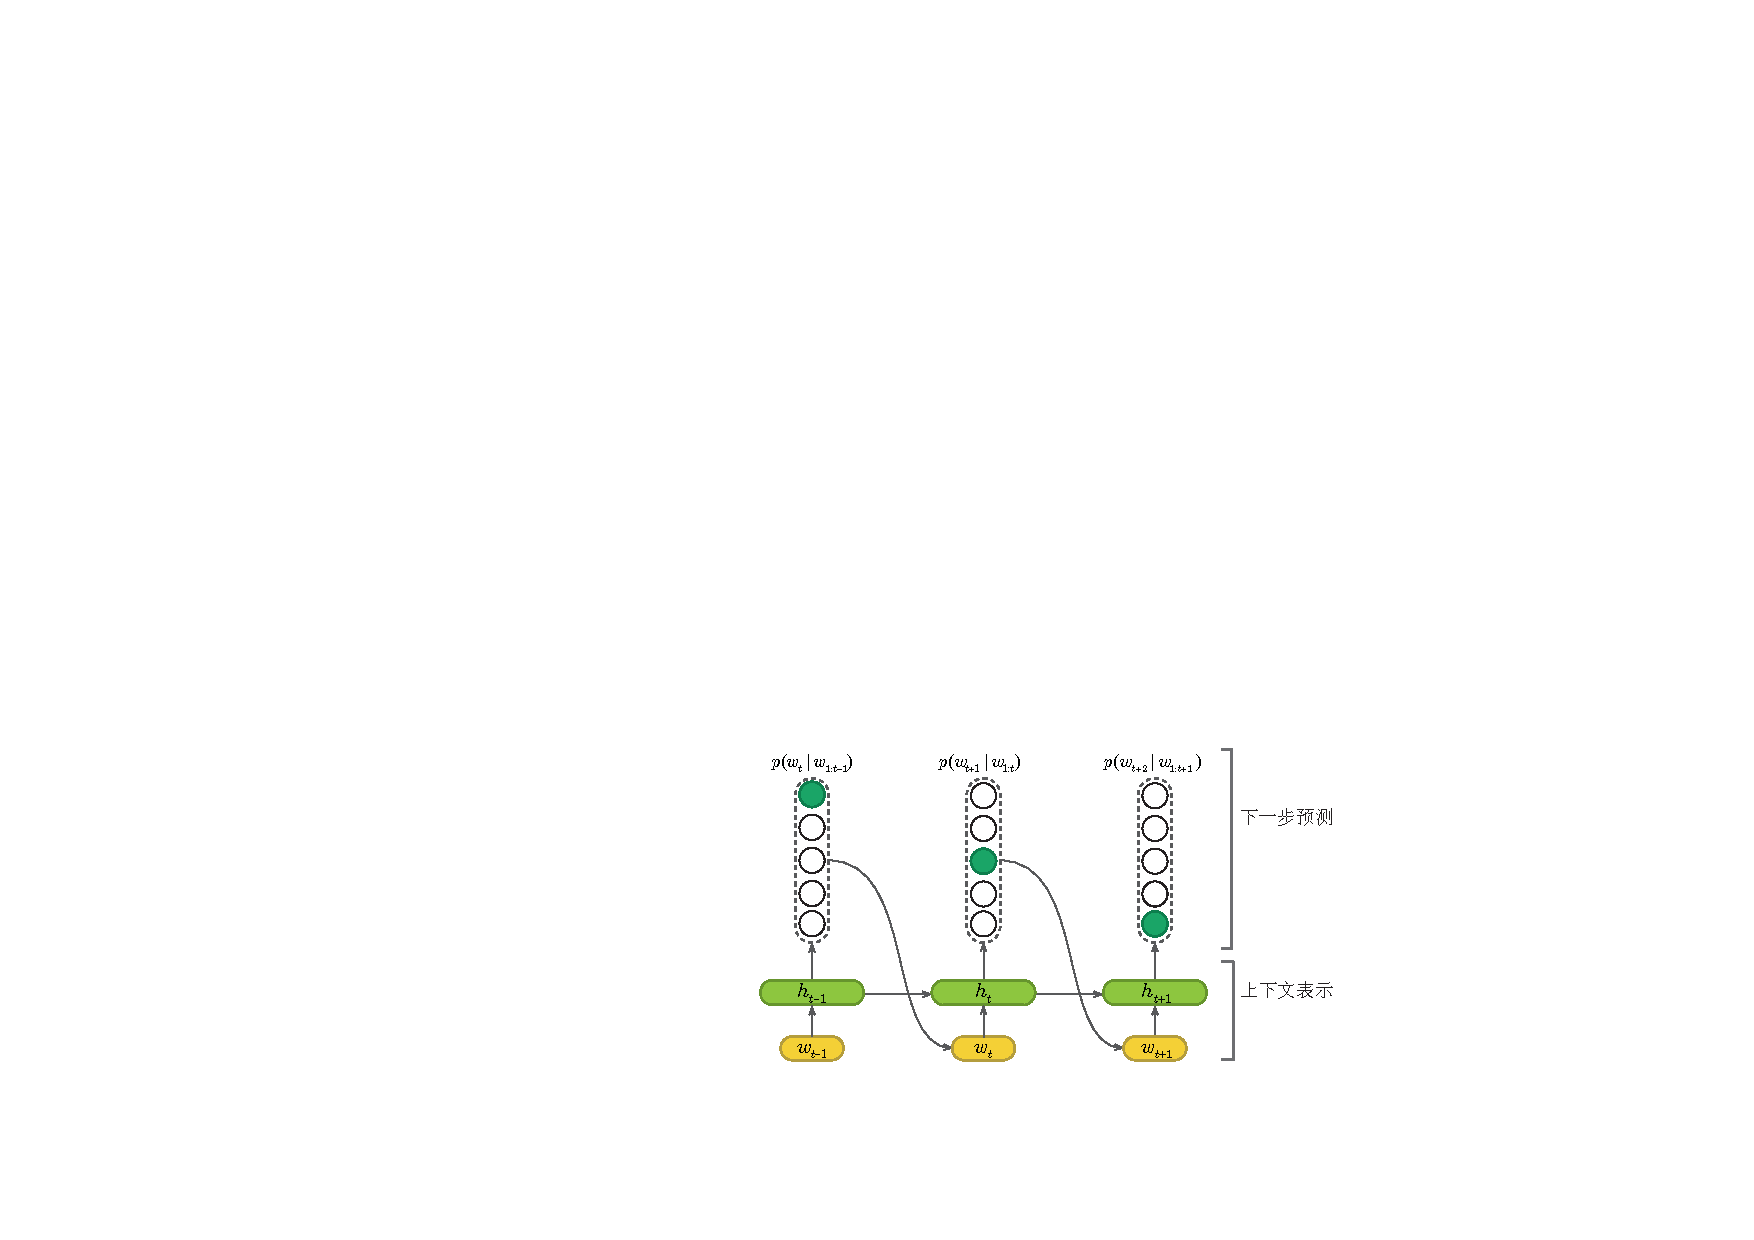
\includegraphics[width=1\columnwidth]{./figures/lm.pdf}
  \caption{循环神经网络语言模型图例}
  \label{fig:lm}
\end{figure}

\subsection{循环神经网络}
所以,考虑到上述长距离依赖问题,本实验采用的基准模型就是基于循环神经网络的语言模型。最近,利用序列的时间序列信息的循环神经网络已经非常流行,如图~\ref{fig:lm}~所示。 为了清楚起见,由于在当前时间步 $ t $的输出$ w_ {t + 1} $正好是下一个时间步的输入$ w_ {t + 1} $,所以没有输出的自动关联连接(Auto-associative Connection)的前一次步骤$ t $回到下一个时间步骤$ t + 1 $中的循环神经网络。每个句子都需要用开始词(即,$ \langle s \rangle $)和结束词(即$ \langle / s \rangle $)标记进行封装。 在预测下一个单词 $ w_ {t + 1} $ 之前,从最后一个隐藏状态$ h_ {t-1} $和当前字$ w_t $接收到循环网络单元的输入。

从形式上讲,循环神经网络是一个参数化的非线性函数$ \mathtt{RNN} $,循环地将一系列向量映射到一系列隐藏状态。 将$ \mathtt{RNN} $应用于任何这样的序列,在每个时间步骤$ t $产生隐藏状态$ h_t $,如下所示:
\begin{equation}
  h_t \leftarrow  \mathtt{RNN}(W\theta^w_t + U h_{t-1} +c),
\end{equation}
其中$ W,U $是模型参数的集合,而$ U $是随时间共享的,向量$ \theta^w_t$ 对应于源词的嵌入$ w_t $。

自Elman提出基本循环网络模型~\upcite{DBLP:journals/cogsci/Elman90}~以来,已经有许多扩展模型提出了克服长距离依赖,梯度消失(Gradient Vanishing)和梯度爆炸(Gradient Exploding)等问题, 如长期短期记忆网络(LSTM)~\upcite{7508408},门限记忆单元(GRU)~\upcite{DBLP:conf/nips/ChungKDGCB15}和近似递归神经网络(Quasi-RNNs)\upcite{DBLP:journals/corr/BradburyMXS16}。

\begin{figure}[!ht]
  \centering
  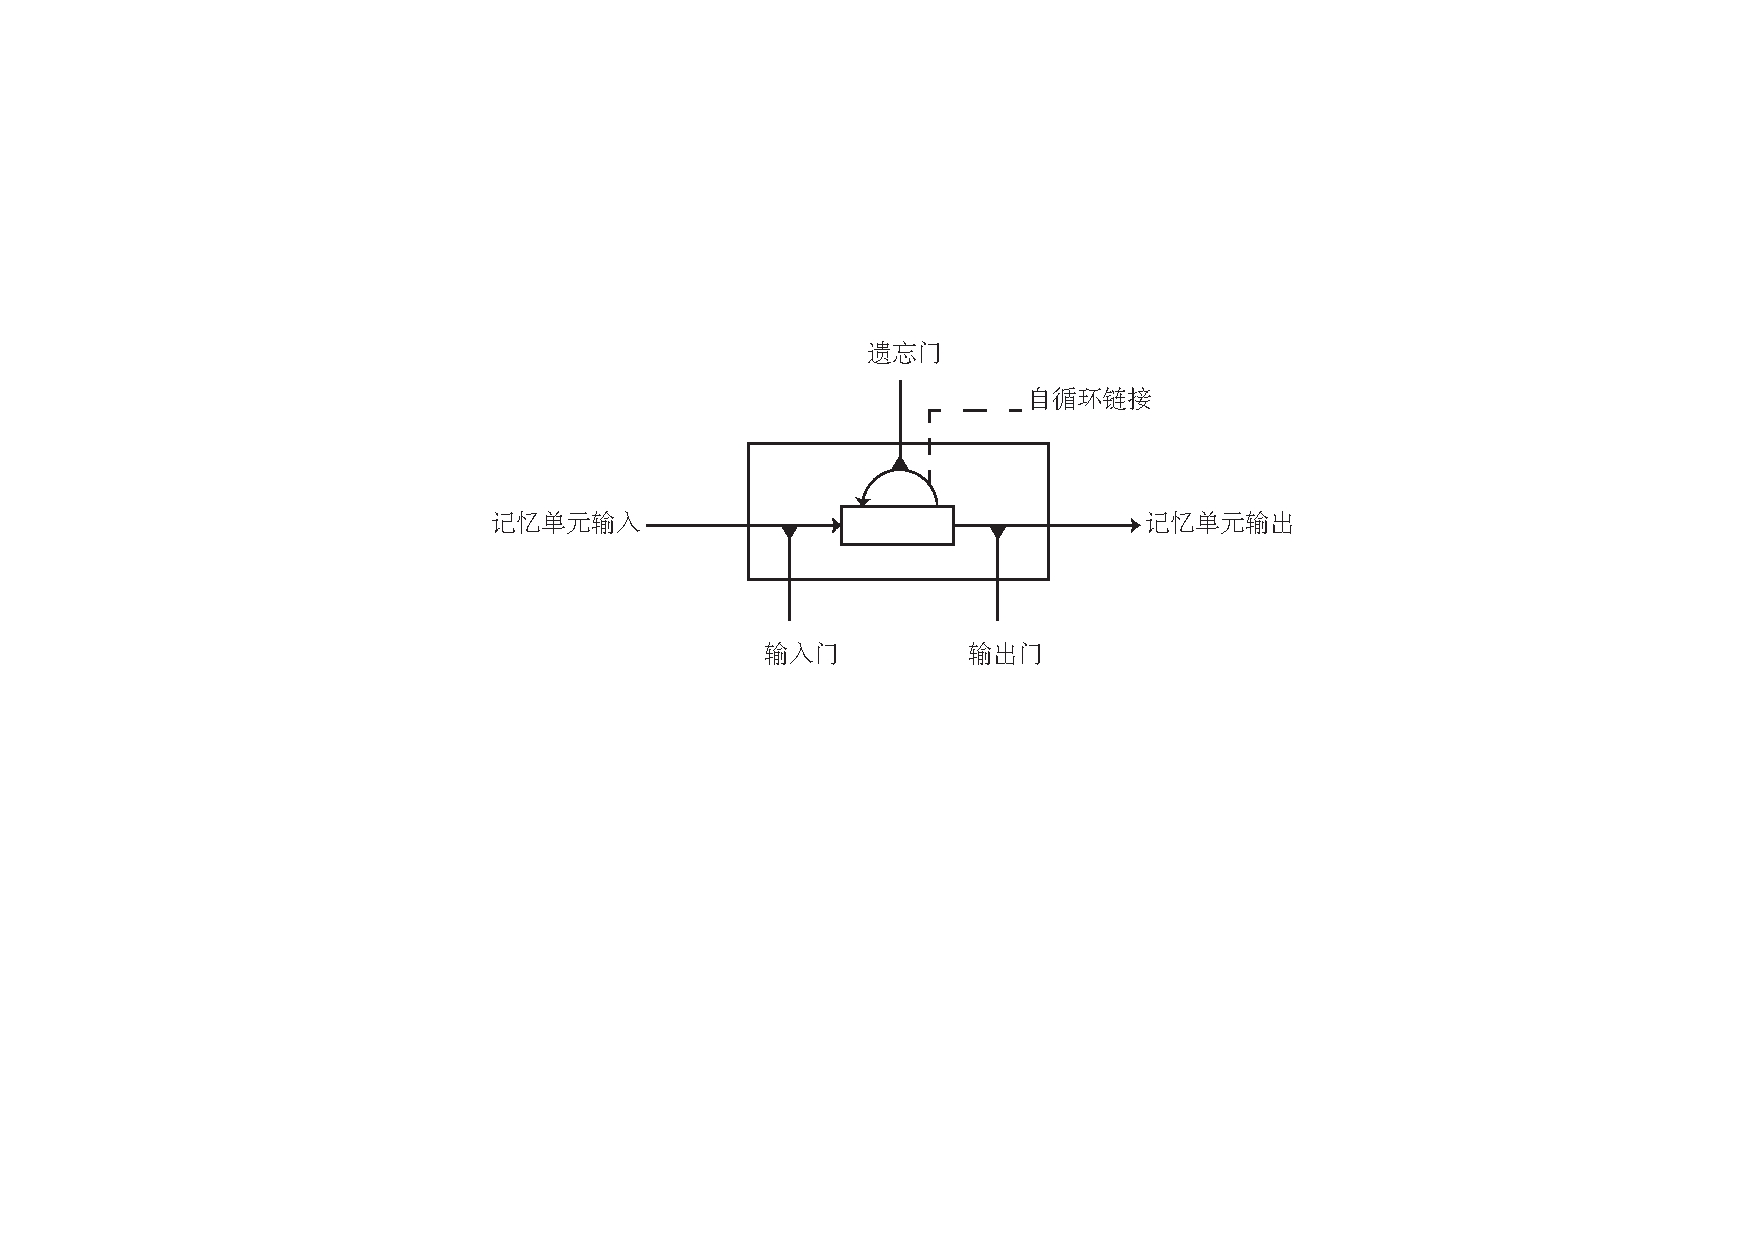
\includegraphics[width=0.7\linewidth]{./figures/lstm.pdf}
  \caption{LSTM 模型示意图}\label{fig:lstm}
\end{figure}

{长距离短期记忆网络}。LSTM的计算公式定于如下 \upcite{DBLP:journals/neco/HochreiterS97}:
\begin{itemize}
\item 输入门。控制当前输入 $x_t$ 和前一步输出 $h_{t−1}$ 进入新的 cell 的信息量:$i_t=\sigma(W^i x_t+U^i h_{t-1}+b^i)$
\item  遗忘门。决定是否清楚或者保持单一部分的状态$f_t=\sigma(W^f x_t+U^f h_{t-1}+b^f)$
\item  变换输出和前一状态到最新状态$g_t=\phi(W^g x_t+U^g h_{t-1}+b^g)$
\item  输出门。计算 cell 的输出$o_t=\sigma(W^o x_t+U^o h^{t-1}+b^o)$
\item  cell 状态更新。步骤:计算下一个时间戳的状态使用经过门处理的前一状态和输入:$s_t=g_t\odot i_t+s_{t-1}\odot f_t$
\item 最终 LSTM 的输出:使用一个对当前状态的 $\tanh$ 变换进行重变换:$h_t=s_t\odot \phi(o_t)$
\end{itemize}
\noindent 其中$\odot$ 代表对应元素相乘(Element-wise Matrix Multiplication), 函数 $\phi(x), \sigma(x)$ 的定义如下:
\begin{equation}\label{equ:tanh}
  \phi(x)=\frac{e^x-e^{-x}}{e^x+e^{-x}},\sigma(x)=\frac{1}{1+e^{-x}}
\end{equation}

{并行计算实现方法}。输入门、遗忘门、输出门和状态更新门矩阵乘法可以并行实现,从而提高LSTM模型的计算效率。因为LSTM的计算模型更容易并行,所以他与GRU的计算时间相差无几,尽管LSTM的模型需要的参数量是GRU模型的1.5倍。
\begin{equation}\label{equ:lstm}
\begin{bmatrix} i^t\\ f^t\\g^t\\o^t \end{bmatrix} =\begin{bmatrix}\sigma\\ \sigma\\\phi\\\sigma\end{bmatrix}\times W\times[x_t,h_{t-1}]
\end{equation}
其中 $W$ 指的是四个小矩阵互相层叠起来 $[W^i,W^f,W^g,W^o]$。




{门限记忆单元。} GRU 可以看成是 LSTM 的变种,GRU 把 LSTM中的 遗忘门和输入门用更新门来替代。 把 cell state 和隐状态 $h_t$ 进行合并,在计算当前时刻新信息的方法和 LSTM 有所不同。 下图是GRU更新 $h_t$ 的过程\upcite{DBLP:journals/corr/Pezeshki15}, 具体定义如下:
\begin{figure}[!h]
  \centering
  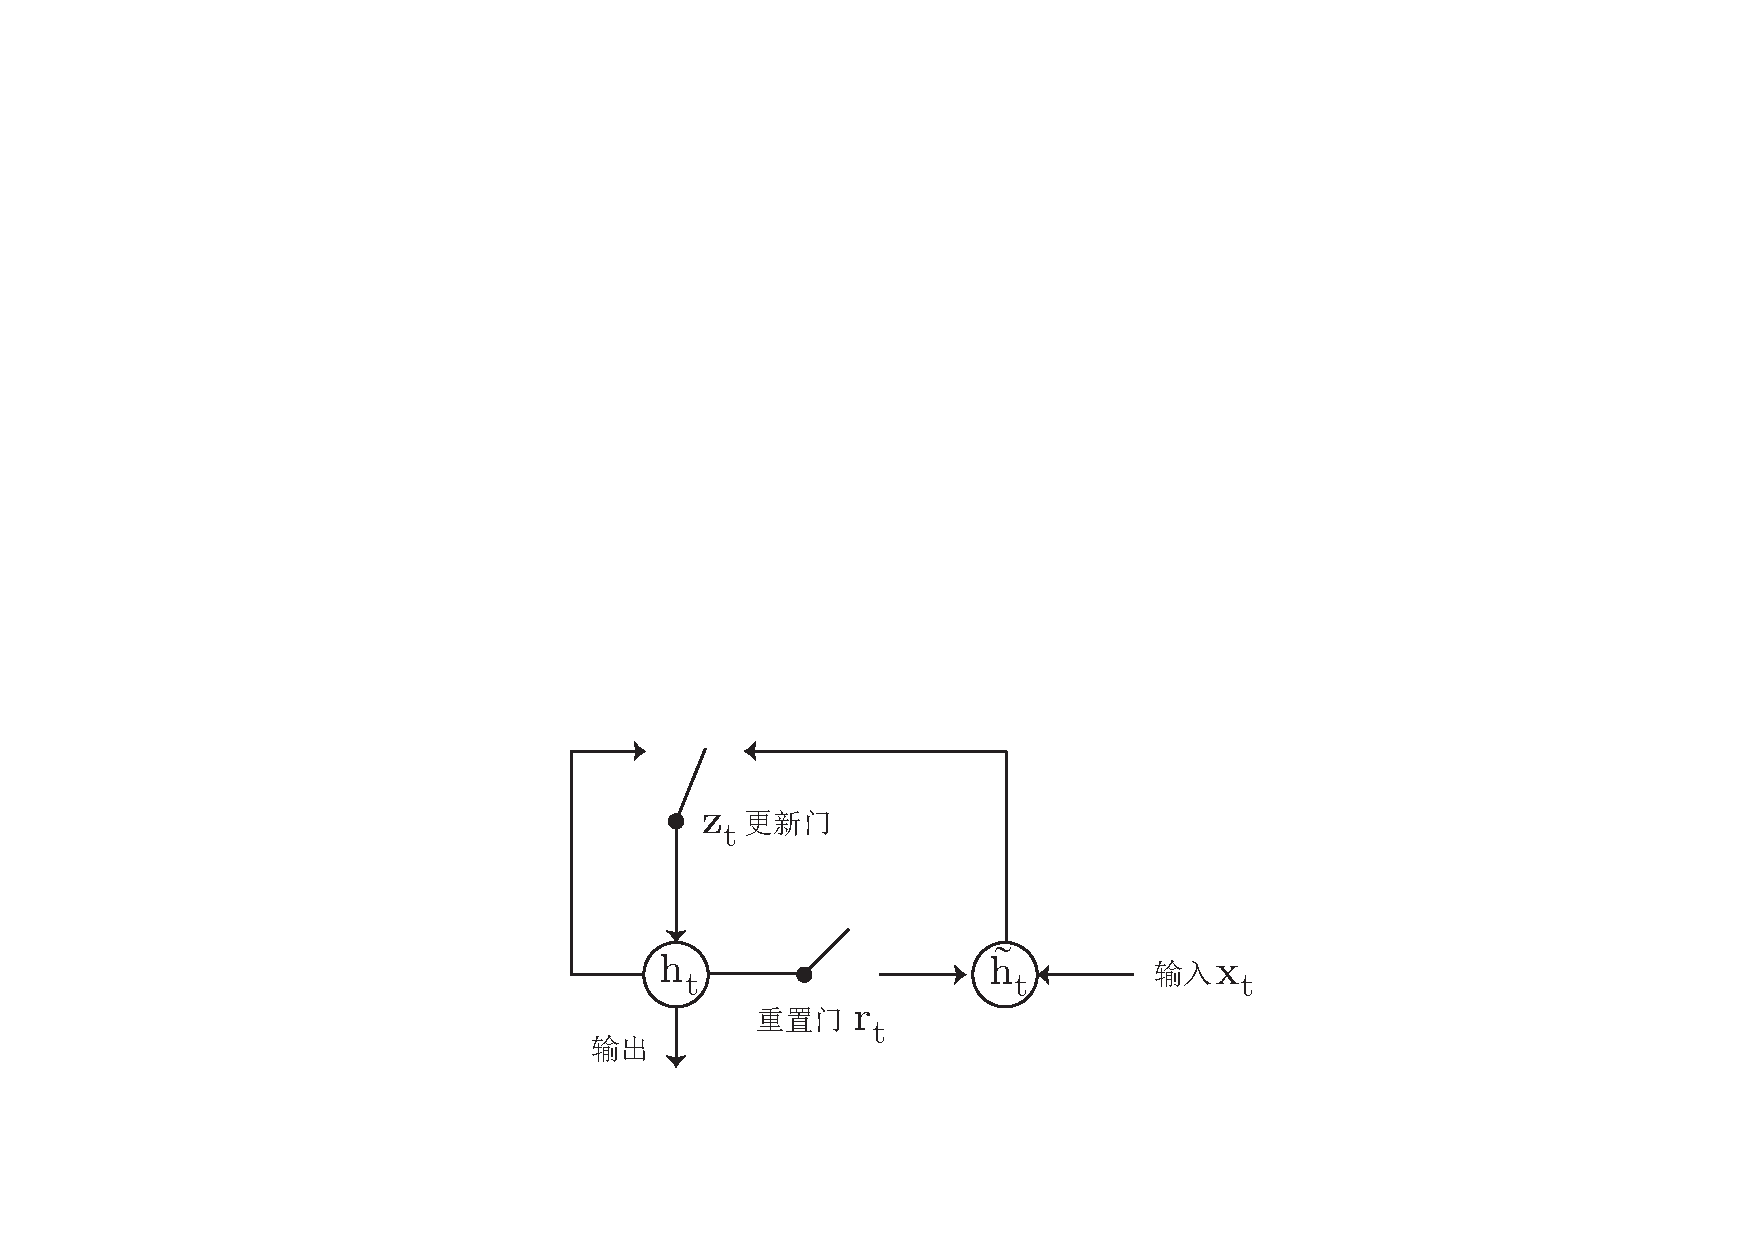
\includegraphics[width=0.45\linewidth]{./figures/gru.png}
  \caption{GRU模型示意图}\label{fig:gru}
\end{figure}

\begin{itemize}
\item 更新门 $z_t$。定义保存多少以前的信息: $z_t = \sigma ( W^z x_t+ U^z h_{t-1}  )$

\item 重置门 $r_t$。 决定保留多少输入信息: $r_t = \sigma(W^r x_t  + U^r h_{t-1}  )$

\item 节点内部更新值$\tilde h_t $。 其次是计算候选隐藏层(candidate hidden layer) $\tilde h_t$,这个候选隐藏层 和LSTM中的$\tilde c_t$是类似,可以看成是当前时刻的新信息,其中$r_t$用来控制需要 保留多少之前的记忆,如果$r_t$为0,那么$\tilde h_t$只包含当前词的信息:$\tilde h_t  = \tanh (W^h x_t  + U^h(h_{t-1} \odot r_t) )$

\item 隐藏层输出值$h_t$。 最后$z_t$控制需要从前一时刻的隐藏层 $h_{t-1}$ 中遗忘多少信息,需要加入多少当前 时刻的隐藏层信息$\tilde h_t$,最后得到$h_t$,直接得到最后输出的隐藏层信息, 这里与LSTM的区别是GRU中没有 输出门:$h_t = (1-z_t)\odot \tilde h_t  + z_t \odot h_{t-1}$
\end{itemize}

如果重置门接近0,那么之前的隐藏层信息就会丢弃,允许模型丢弃一些和未来无关 的信息;更新门 控制当前时刻的隐藏层输出$h_t$需要保留多少之前的隐藏层信息, 若$z_t$接近1相当于我们之前把之前的隐藏层信息拷贝到当前时刻,可以学习长距离依赖。 一般来说那些具有短距离依赖的单元重置门比较活跃(如果$r_t$为1,而$z_t$为$0$ 那么相当于变成了一个标准的RNN,能处理短距离依赖),具有长距离依赖的单元更新门比较活跃。



\section{大词表问题}
作为多标签分类(Multi-class Classification)的标准概率归一化方法,对于大词表问题中,\texttt{log-softmax} 函数和相应的梯度(Gradient)可以定义为:
\begin{equation}
\begin{split}
p(w|h)=&\frac{\exp(h^\top v_{w})}{\sum_{w_j\in \mathcal{V}}{\exp(h^\top v_{w_j} )}} \\
\frac{\partial p(w_i|h)}{\partial v_{w_j}}=&p(w_j|h)(\delta_{ij}-p(w_i|h))h^\top\\
\end{split}
\end{equation}
\begin{equation}
\label{eq:softmax}
\begin{split}
\log p(w|h) &= \theta^w h-\log \sum_{u\in \mathcal{V}}{\exp(\theta^u h)}\\
\nabla_{\theta^u}{\log p(w|h)}&= (\delta_{uw}-p(w|h))h
\end{split}
\end{equation}
其中$ h $是隐藏层输出的向量(即上下文表示),$ \theta ^ w $表示单词$ w $的目标单词嵌入~\upcite{duda2012pattern}。 同样对于克罗内克 $\delta$ 函数$ \delta_ {uv} $(Kronecker Function),如果$ u,v $指代的是相同的单词结果是$ 1 $,如果$ u,v $指代的不是相同的单词则是$ 0 $。


如等式~\ref{eq:softmax}~所示,前向概率传播函数$\log p(w|h) $(即第一行方程)和后向梯度优化函数$\nabla_{\theta^u}{\log p(w|h)}$(即第二行的方程)都需要计算目标词汇表中的所有单词,因此在这个部分上花费的时间会随着词表中包含的单词数量的增加而线性增长。对于包含$ \mathcal{| V |} $ 数量的单词来说,总的时间复杂度是$ \mathcal {O}(\mathcal {| H || V |})$,其中$ \mathcal {| H |} $表示隐藏层输出的维度。即使对于采用现代通用计算体系结构的GPGPU来说, 尽管其非常适合于具有高计算并行的矩阵乘法,这种计算负担也是相当高的。因此,采用现代硬件体系结构的训练和推理中,输出字嵌入矩阵的超大尺寸仍然是一个计算瓶颈。而且,目前的设备的显存是有限的,不能任意增大显存大小,所以对词表大小有一个天然的上限。

值得注意的是,\texttt{softmax} 算法的瓶颈不能归因于``for''循环函数(即方程~\ref{eq:softmax}~)中的$ \sum_ {u \in \mathcal {V}} $,尽管它随着词汇量的增长而线性增长,但是矩阵张量的乘法计算的规模较大。因为矩阵计算需要更多的时间来获得结果,但线性求和可以更快地计算完成。所以,相比于``for''循环函数而言,主要的计算时间用于矩阵乘法计算。我们在这里说明的目的是,只有那些避免其他冗余字的计算概率才能达到边际加速比的方法,而那些仍然涉及全局概率规一化的方法,实际上并不能真正改善这个部分的计算占用的时间。

%其中由于分母是正则项,一旦词表扩大,每次迭代更新都需要计算这一项,是主要的问题所在,所以本课题拟在主要解决该问题所导致的计算费时的问题,

因此,在保证计算精度不下降的情况下,我们期望能缓解计算概率归一化项的计算瓶颈并且提高模型的训练速度。 目前主要缓解大词表问题的算法主要分为以下三类: 单词拆分算法(Vocabulary Truncation)、采样估计模型(Sampling-based Approximation)和层次分解模型(Vocabulary Factorisation)。下面我们将一一详述。


\subsection{单词拆分算法}
针对大词表问题的解决方法,最直接最简单的策略就是我们放弃使用大词表,转而保留一个较小的词表来保证训练的内存占用小和计算效率高。那么针对剩余的过多的词表外的单词(Out-Of-Vocabulary,OOV),我们可以使用传统的N-gram语言模型来估算其可能的概率分布。这样做一方面保证神经网络模型可以在有限时间内训练完,同时保证模型的最后的测试结果不会很差~\upcite{DBLP:journals/csl/Schwenk07}。

然而我们需要注意到,当我们的词表继续减少和我们的所有单词种类不断变多的时候,我们会发现训练样本中存在过多的$\langle$unk$\rangle$ 字符,这样使得神经网络的模型训练非常困难,进而导致模型效果变得非常地差,所以这种方案只是一定程度上缓解了大词表问题,但是也是一种有效的尝试方案。

除了上述直接的建模方案外,目前采用的方案是将单词按照字符级别来划分,可以将一个单词按照字符统计规律划分成任意多个子词。其中二元对编码(byte-pair-encoding,BPE)能将一个单词划分成两部分:前缀(Prefix)和后缀(Suffix)~\upcite{DBLP:conf/icassp/Tucker0P94, DBLP:conf/acl/SennrichHB16a,Gage:1994:NAD:177910.177914},如图~\ref{fig:subword} 所示。从该图中我们可以看出,单词被划分成前缀和后缀两部分,其中$+$代表是单词的前缀,同时$\langle /w \rangle$是单词的后缀。由于划分规则是从训练数据中学习到的,我们可以指定需要缩减的词表大小,所以该算法的动态适应性很强,目前主流的机器翻译模型都采用这个方案~\upcite{DBLP:journals/corr/JozefowiczVSSW16}。尽管如此,我们仍然需要看到它这样的解构操作依然带来了一定的损失,因为句子的长度加倍了,对RNN的长距离关系学习能力提出了更高的挑战~\upcite{DBLP:conf/aaai/KimJSR16}。

\begin{figure}[!h]
  \centering
\includegraphics[width=0.6\linewidth]{./figures/subword.pdf}
\caption{词到子词划分样例}\label{fig:subword}
\end{figure}

\subsection{采样估计模型}
目前采用的采样算法(Sampling Algorithm)主要是针对公式~\ref{eq:softmax}~中对所有单词概率规约那一项进行概率估计,其中著名的算法有:重要性采样(Importance Sampling)~\upcite{DBLP:journals/tnn/BengioS08},噪声差分估计(Noise Contrastive Estimation, NCE)~\upcite{DBLP:conf/icml/MnihT12}和Blackout 采样算法~\upcite{DBLP:journals/iclr/JiVSAD15}。第一种算法在Bengio的实验中被证明模型无法收敛~\upcite{DBLP:journals/tnn/BengioS08},因此目前主要使用的后面两种算法。

对于NCE噪声差分估计算法来说,模型需要学习将正确的单词 $w_0$ 与随机生成的单词 $\{w_1\cdots w_k\}$做一个二元分类。 其中 $w_0$ 训练样本中真正的下一个单词, $\{w_1\cdots w_k\}$ 是采用先验分布  $q(w)$产生的随机噪声单词. 正例归一化后的概率和所有负例联合概率的公式可以写成:
\begin{equation}\label{equ:nce}
\begin{split}
  \tilde{p}(y=1|h)=&\frac{\exp( \theta^w_0 h)}{ \exp( \theta^w_0 h)+k *q(w_0)}\\
  \tilde{p}(y=0|h)=&\prod_{i=1}^{k}\frac{k *q(w_i)}{\exp( \theta^w_i h)+k *q(w_i)}\\
\end{split}
\end{equation}
需要注意的是噪声概率 $\tilde{p}(y=0|h)$ 需要对 $k$ 个噪声样本做加法运算而不是对整个词表单词进行的。 这样的话该算法的计算机复杂度就是$\mathcal{O}(k+1)$,和整个词表的大小无关了。从而该算法的加速比是$\mathcal{O}(\mathcal{|V|}/(k+1))$

除此之外,最近提出的Blackout采样算法针对噪声概率归一化的时候与当前上下文的相关,对上述的NCE算法进行了进一步优化和修正~\upcite{DBLP:journals/iclr/JiVSAD15},同时也引入了更多的计算量。其模型的代价函数计算公式定义为:
\begin{equation}
\begin{split}
  \ell=&-\log(p(w_0|h)) - \sum_{w_i \sim p(w)} \log(1 - p(w_i))\\
p(w_i) =& \frac{\exp(\theta^w_i h)}{\sum_{w_i \sim p(w)} \exp(\theta^w_i h)}.
\end{split}
\end{equation}

总的来说,这些采样近似算法可以显着加快训练速度,但仍然需要时间来利用单词分布$q(w)$~\upcite{DBLP:conf/naacl/ZophVMK16}来采样大量的噪音单词,采样单词足够多的情况占用的时间仍然很客观,需要进一步手段优化。 另一方面,Softmax函数在推理测试的时候必须要计算,意味着在测试推理的时候该算法失效了。因为候选词是在整个词汇表中预测的,而不仅仅对当前的采样的早噪声单词做预测,而且我们更无法得知正确的单词是什么\upcite{DBLP:journals/jmlr/GutmannH12}。

这里我们需要注意的是,由于我们引入了采样函数$q(w)$,模型会花费额外时间在采样计算上面。从离散分布采样的初始程序通常需要词汇数量具有线性时间复杂度。因此我们需要寻找一个性能优异的带权重的随机数生成器或者是离散采样函数。


\subsection{层次分解模型}
层次分解方法,可以大大降低学习和推理过程中表示概率分布的所占用的计算内存,因为它只计算局部概率并且选择每一层的分数最高的候选路径而不是保存全局计算结果。
目前主要的分解策略可以分为: 基于类别的多元分类模型(class-based hierarchical softmax, cHSM)和基于二叉树的二元分类模型(class-based hierarchical softmax, tHSM)。接下来我们将这两种算法的详细计算过程进行描述。

首先我们考虑基于类别的分解策略。假设语料中的每一个词样本属于且只属于一个类(class或者group),在此基础上计算词样本在语料中的分布时,可以先计算类的概率分布,然后在所属类上计算当前词的概率分布,于是可将公式~\ref{eq:softmax} 转化为:
  \begin{equation}
  \begin{split}
p(w|h)=&p^c(\mathcal{C}(w)|h)\cdot p^w(w|\mathcal{C}(w),h) , w\in \mathcal{C}(w),\\
&\mathcal{V}=\bigcup _{i = 1}^\mathcal{C}{c_i},\quad  c_i \bigcap c_j=\phi, \text{若}\quad i\ne j, \\
\end{split}
\end{equation}
其中 概率~$p^c(\mathcal{C}(w)|h)$~表示每个类别的概率,$p^w(w|\mathcal{C}(w),h)$~表示在类别$\mathcal{C}(w)$中所有单词的局部概率。

此时,训练一个词样本的计算复杂度正比于: $\mathcal{O =|H||C|}$。 在该计算公式中,$\mathcal{C}$ 为语料中所有词的分类数,可根据语料中词的词频进行划分。 当$C$ 取$1$ 或取词典大小$|V|$ 时,此结构等同于标准的Softmax 结构,此时词表还是原来的结构,并没有任何优化效果。因此,对于绝大多数情况,我们取$\mathcal{C} \ll \mathcal{V}$并且 $|\mathcal{C}|\ll 1$,这样的结构才能保证有效降低 softmax 的计算复杂度。图~\ref{fig:case_hsm} 展示了类别划分和分步概率计算的示例。从图中我们可以得知,其中词表 [duck,cat,mop,broom] 被划分成两个类别:$c_1\to$[duck,cat],$c_2\to$[mop,broom]并且$c_3\to$[the,am]。
\begin{figure}[!h]
  \centering
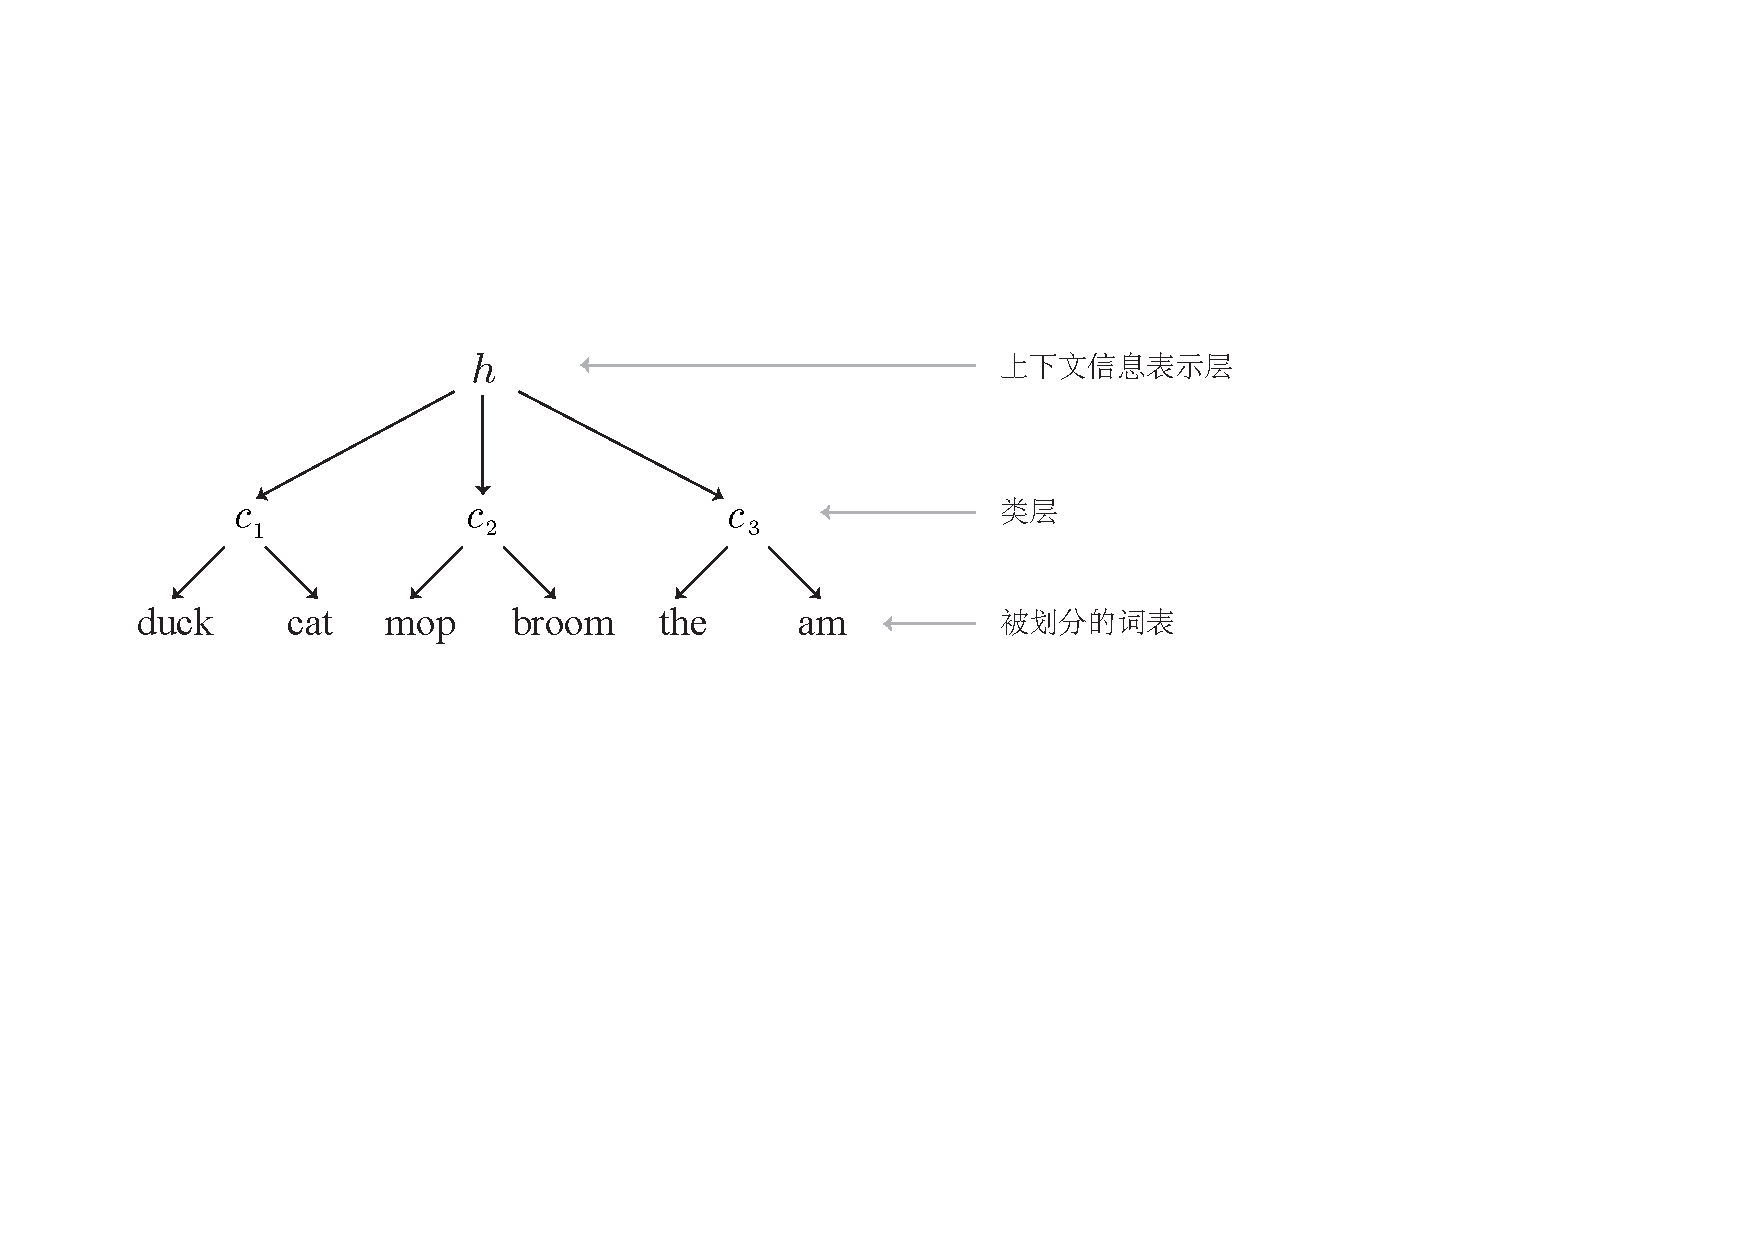
\includegraphics[width=0.79\linewidth]{./figures/case_chsm.pdf}
\caption{cHSM算法可视化模型}\label{fig:case_hsm}
\end{figure}

假设每个类包含 $\sqrt{\mathcal{|V|}}$ 单词,表示词汇被划分为相同大小的组,这样的话级联概率(cascaded probability)只涉及$2\sqrt{\mathcal{|V|}}$ 单词 softmax计算,所以最优时间复杂度可以减少到$\mathcal{O}(\mathcal{|H|}\sqrt{\mathcal{|V|}})$~\upcite{DBLP:conf/icassp/Goodman01}。虽然在更常见的情况下,分区算法会产生不同大小的字组,这需要外部的其他结构来建立高效的数据结构,并且这些稍微复杂的算法尚未被完全探索和分析。此外,我们还可以通过不同的类大小和分区算法来调整精度和效率之间的权衡关系。

另一方面,我们再介绍基于二叉树分解词表的建模策略。tHSM方法将一步多类分类分解为多个二元分类步骤。正因为如此,词汇组织为二叉树,其中单词分布在二叉树的叶子节点上,二叉树的所有的中间节点的都是内部参数。如果该二叉树是平衡树的结构情况下,每个词将会被赋予相等长度的前缀,最优时间复杂度可以减少到$\mathcal{O(|H|\log \mathcal{|V|})}$。最早的工作中,单词在二叉树上的分布可以由WordNet与人类专家~\upcite{DBLP:conf/aistats/MorinB05}或单词 unigram 分布~\upcite{DBLP:conf/nips/MikolovSCCD13}的霍夫曼编码构建。然而,在现实世界的大规模文本应用中,专家知识的构建是相当昂贵的。所以,一般人们也不会采用这样的方案来构建单词的二叉树分布。霍夫曼编码方案只考虑单数据统计,而单词的语境,句法或语义信息尚未被考虑和得到彻底的讨论。

\begin{figure}[!h]
  \centering
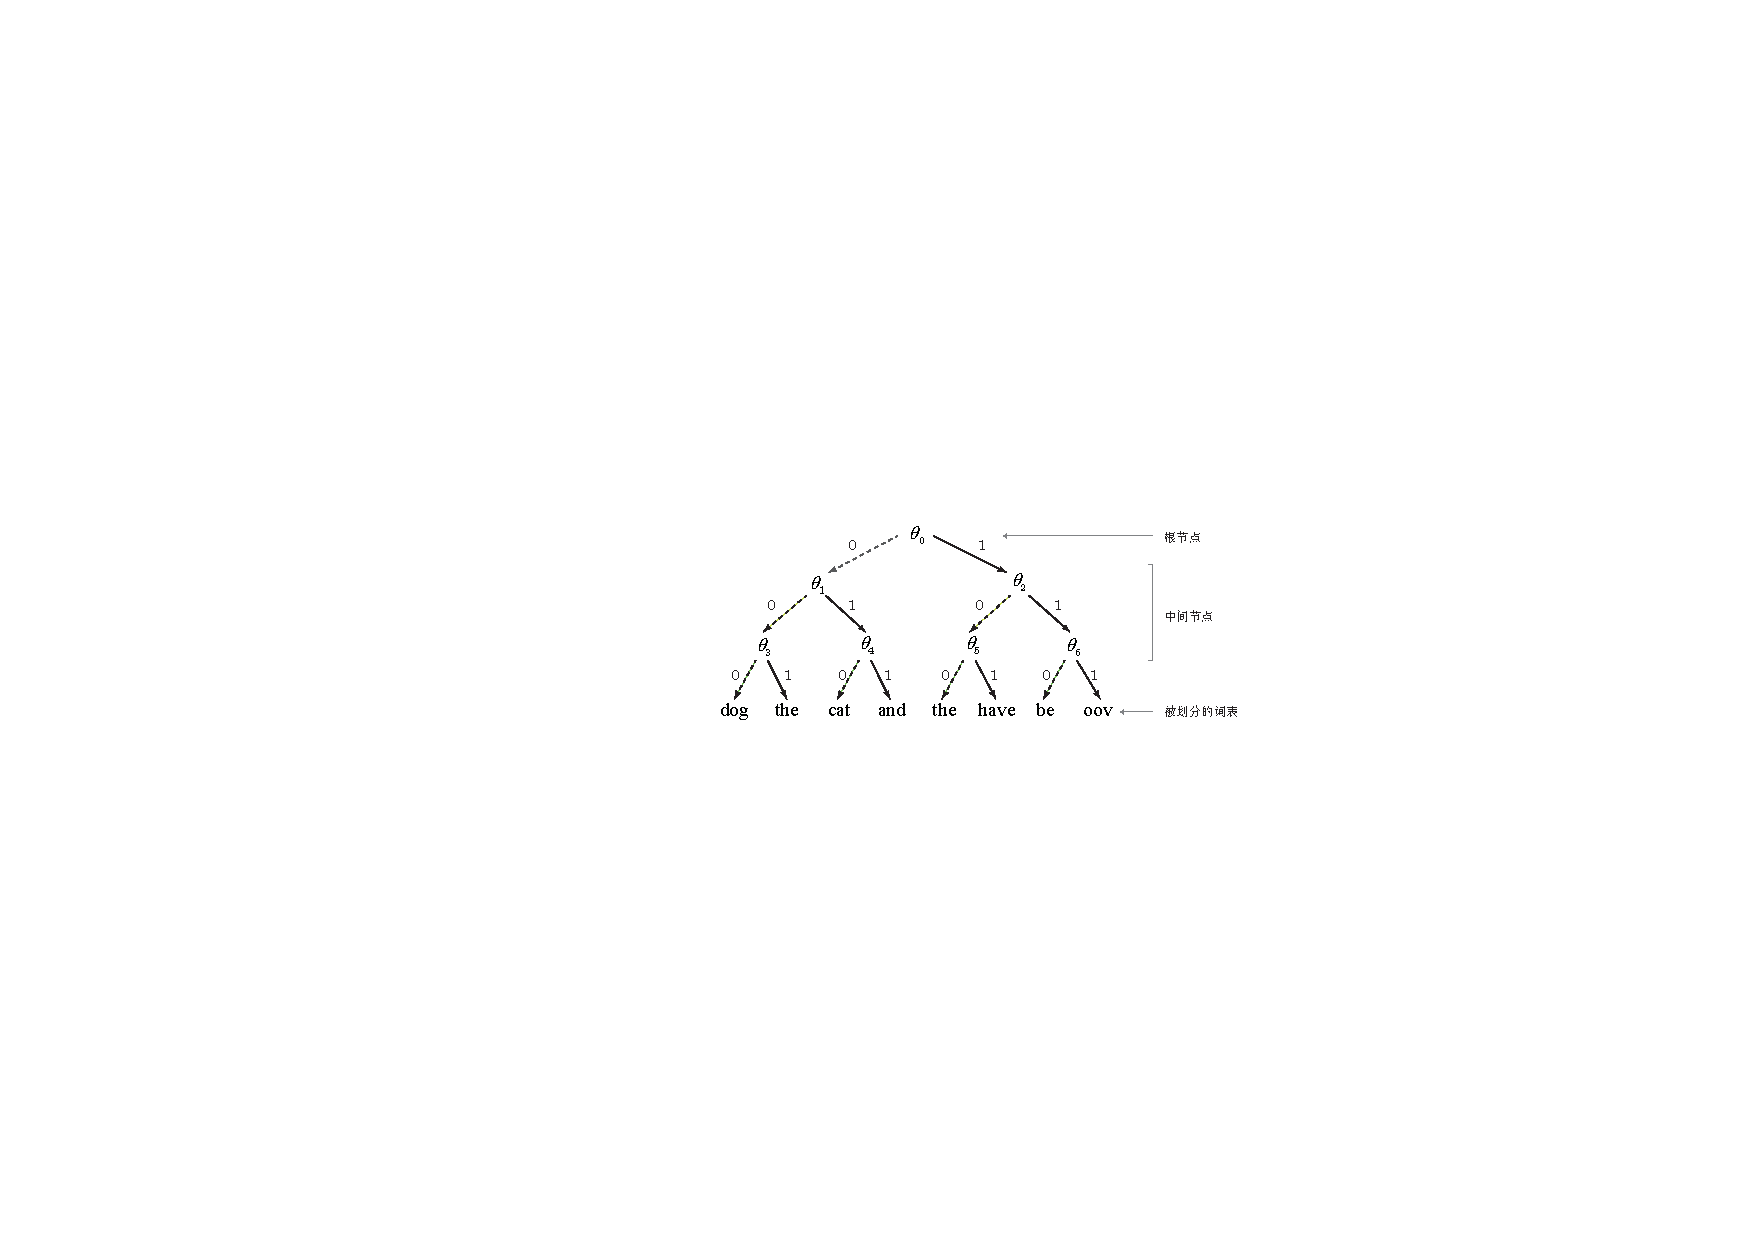
\includegraphics[width=0.9\linewidth]{./figures/thsm-example.pdf}
\caption{tHSM算法可视化模型}\label{fig:case_thsm}
\end{figure}

图~\ref{fig:case_thsm} 展示了二叉树概率分解和计算的示例。

Mikolov当年曾提出使用基于二叉树的层级softmax模型来加速的训练方案,加速比能达到理论的最大速度。但是需要注意的是,当时提出的背景是基于CPU计算方案构建的,如今随着应用领域的推广越来越多的算法应用到实际问题中,我们需要在并行度更高的GPU上进行计算,因此基于GPU进行建模的tHSM和历史上研究众多的cHSM算法尚未被研究提及,因此我们将会需要在本文中详细研讨。

\section{离散采样算法}
在我们使用基于采样的模型时,我们不可避免的需要使用到离散采样函数,即:设一共有$|\mathcal{V}|$个单词,第$i$个单词出现的概率是$p(w_i)$, 如何高效地产生这样的随机变量序列$w_1,w_2,\cdots$?

这问题其实正式来说,可称为模拟离散取样(Simulated Discrete Sampling),跟据有限类别的指定的概率,来模拟取样,生成采样序列输出。其中,要制造指定的概率分布随机变量,关键就是如何通过均匀分布变换获得。因为我们的计算机只能快速产生伪随机数,即均匀分布的采样输出。其他的复杂采样函数均建立在均匀分布的变换之上。
\subsection{随机采样函数}
当我们使用概率模型实现推理和学习算法时,通常需要从离散分布进行抽样。 也就是说,从参数$\boldsymbol {\pi} \in \mathbb{R} ^ K$中的多项式分布,使得$\ pi_k \geq 0$和$\sum_{k} \pi_k = 1$。 更常见的情况是我们在$\mathbb{R}^K$中有一个$\boldsymbol {\phi}$ ,其中$\phi_k \geq 0$,但我们不知道规范化常量。 也就是说,$\boldsymbol{\pi}$只与多项式参数$\boldsymbol {\pi}$成正比。 我们希望根据$\boldsymbol{\pi}$快速生成一个变量,给出$\boldsymbol {\pi}$,用(Matlab)代码很容易地完成某些操作:
\begin{verbatim}
cdf = cumsum(phi);
samp_k = sum(cdf < rand()*cdf(end)) + 1;
\end{verbatim}
这很好很简单,但是你会注意到它具有每个样本的设置(计算CDF)和$\mathcal {O}(K)$时间复杂度的$\mathcal {O}(K)$时间复杂度。每个样本的复杂度可能被降低到$\mathcal {O}(\log K)$,找到阈值的数据结构更好。事实证明,我们可以做得更好,得到$\mathcal {O}(K)$的抽样,而仍然是$\mathcal {O}(K)$。
\subsection{基于线性搜索的逆变换方法}
在上节中,显示了CDF的一些特性,例如CDF的范围是$[0,1]$,而且是一个单调递增的(Monotonic Increasing)函数。逆变换取样算法(Inverse Transform Sampling)就是利用了这些特性,来解决上面提出的问题。其实,逆变换取样方法并不是很复杂,我们接下来详细解释。给一个目标CDF,只要计算其逆函数(Inverse Function),就可以把均匀的随机变数转换为目标CDF:
\begin{equation}\label{equ:func}
  X=F_X^{-1}(Y)
\end{equation}

这方法能用在所有CDF(包括连续及离散的)。其数学证明可参考维基百科。

下图显示这个方法的直观解读,在Y轴范围$[0,1]$里均匀取样$(y_i)$,之后向右和CDF取交点,求交点的$X$轴位置($x_i$),$X$则是符合CDF的概率分布。这个方法用在离散的情况就更简单,只需搜寻目标的CDF,找出超过均匀取样的元素即可。
\begin{figure}[!h]
  \centering
\includegraphics[width=0.5\linewidth]{./figures/cdf.png}
\caption{累计函数采样方法示意图}\label{fig:cdf}
\end{figure}
在离散的情况下(本文题目要求),其时间复杂度是O(N),其中N为类别数目。

读者可能会注意到,这里用了线性搜寻(Linear Search),如果targetPdf数组是由大至小排列,平均而言会更快找到结果。另外,也可以用二分搜寻(Binary Search),那么复杂度会降低为$O(\log |\mathcal{V}|)$,。


\subsection{基于二叉树搜索的逆变换方法}
二分搜索(binary search),也称折半搜索(half-interval search)、对数搜索(logarithmic search),是一种在有序数组中查找某一特定元素的搜索算法。搜索过程从数组的中间元素开始,如果中间元素正好是要查找的元素,则搜索过程结束;如果某一特定元素大于或者小于中间元素,则在数组大于或小于中间元素的那一半中查找,而且跟开始一样从中间元素开始比较。如果在某一步骤数组为空,则代表找不到。这种搜索算法每一次比较都使搜索范围缩小一半。

事实上,这个问题用二分搜寻是标准的方法。那么,还有没有更快的方法呢?答案是肯定的,例如别名方法(alias method)、近似方法等~\upcite{DBLP:journals/cgf/ClineRW09}。当然,在N很小的情况下,线性搜寻和二分搜寻也足够。
\subsection{别名方法}

设$ Z $为离散的随机变量,它有n个可能的结果$ z_0,z_1,\ldots,z_ {n-1} $。 为了简化下面的讨论,我们研究另一个变量$ Y $,其中$ P \{Y = i \} = P \{Z = z_i \} $。 当$ Y $取值$ i $时,让$ Z $为$ z_i $。 所以$ Z $可以从$ Y $生成。随机变量$ X $被均匀分布在$(0,n)$中,这个概率密度函数是
\begin{equation}\label{equ:alias}
 f(x) = \left\{
 \begin{array}{rl}
  1/n & \text{若 } 0 < x < n\\
  0 & \text{否则}\\
 \end{array} \right.
\end{equation}
那么我们现在生成的$Y'$是:
\begin{equation}\label{equ:gen}
  Y' =  \left\{
 \begin{array}{rl}
  \lfloor x  \rfloor & \text{若 } (x - \lfloor x \rfloor) < F(\lfloor x \rfloor)\\
  A(\lfloor x \rfloor)  & \text{否则}\\
 \end{array} \right.
\end{equation}
其中$ A(i)$是别名函数。 当$ x $落入范围$ [i,i + 1)$($ i $是一个整数)时,$ y $的概率$ F(i)$为$ i $,概率$ 1 - F(i )$是$ A(i)$。 由于$ x $是均匀分布的,
\begin{equation}
  \begin{split}
P\{x \in [i, i + F(i))\}     &= \int_i^{i+F(i)}\frac{1}{n}dx= (i + F(i) - i) \times 1/n= F(i)/n,\\
P\{x \in [i + F(i), i + 1)\} &= \int_{i+F(i)}^{i+1}\frac{1}{n}dx= (i + 1 - (i + F(i))) \times 1/n= (1-F(i))/n
\end{split}
\end{equation}

让我们将满足$ A(j)= i $的值集合$ j $表示为$ A ^ { - 1}(i)$。 生成的变量$ Y'$具有以下概率质量函数:
\begin{equation}
  P\{Y' = i\} = F(i)/n + \sum_{j \in A^{-1}(i)}\frac{1-F(j)}{n}
\end{equation}
Alias方法是构造$ A $和$ F $的算法,所以$ P \{Y'= i \} $等于$ P\{Y = i \} $。 由于$ A $和$ F $的域都是整数$ 0,1,\ldots, n-1 $,所以它们可以存储在数组中,并且可以在$O(1)$中查找值,其中空间效率是 $\mathcal{O}(n)$。

虽然别名方法可用于生成丰富的噪声字,因为它需要线性建立时间和恒定的采样时间~\upcite{10.2307/2683739,DBLP:conf/emnlp/VaswaniZFC13}。

大词表问题,主要是对softmax如何建模的问题。在本课题中,我们探讨 cHSM 和 tHSM 两种不同的方案所带来的影响和优劣。
\section{本章小结}
本章对国内外学者在语言模型的任务上相关工作进行了介绍。首先,介绍了语言模型的建模策略和对应的应用方案。并详细讨论了循环神经网络的语言模型的建模方式,并讨论了其结构的优缺点。同时为了解决使用循环网络所带来的梯度爆炸的问题,我们进而引入了长距离短期神经网络和门限记忆节点两种基于门限机制的循环网络;另一方面,我们还考虑了语言模型大规模应用所带来的大词表问题,并作了详细分析其原因。为了解决该问题,我们还讨论了历史上所提出的方案,并做了分类讨论。主要涉及三种思路:缩减词表大小,用采样算法近似估计和模型层次分解。针对各种模型提出的结果做了详细介绍,并分析了各种算法的优劣处。最后我们分析了实验中需要用到的高效采样函数的构造算法。
\chapter{模型}
在文献中,源词和目标词分别被称为模型的输入和输出。源词通常可以用分布式表示来表示,称为输入词嵌入(Word Embedding),可以使用基于外部语料库的连续词袋模型或Skipgram模型来训练。而这两个模型来源于语言模型任务,并且为了在特征空间中产生可能的嵌入分布而被大大简化。另外,输出字通常表示为字索引(Indexing)或1-K编码,并且可以与softmax概率函数直接关联。

在本节中,我们将这个目标词表示扩展到一个分层的形式,使它们适配基于类和基于树的分层概率计算。首先,我们提出了一个在分层结构上建模参数的字编码方案。因此,考虑到GPU上的并行吞吐性能,我们推导出紧凑的代价函数及其梯度。同时,类或树上的单词分布对其性能有很大的影响,应该在训练阶段之前定义,这些动态交换算法在训练过程中改变了单词群或子树结构在这个研究中。我们采用了几个分层聚类和词汇分割策略,用统计,句法和语义知识来初始化其结构,以达到一个稳定和可以预期的性能。而且,在推理过程中,不同于传统的softmax情况,得到最好的候选者自然是可行的,层次推理不能直接用 softmax 方法来实现。我们讨论基于树和基于类的搜索策略的两种不同的推理情况:a)打分:输出给定序列的概率;b)排序   :在给定的上下文中获取得分最高的一个候选单词。
\section{模型一}
\subsection{基于二叉树的单词编码}
在叶子上有文字的二叉树的情况下,我们可以通过访问从根到叶的所有内部节点来定位每个特定的词。在这里,单词$ w $的路由表示所有内部节点$ \theta^w_i $和它访问的边缘$ d ^ w_i $。

为了说明,$ \theta_i ^ w $表示到达单词$w$的路径上的$ i^{th} $层上的非叶节点,并且$\mathbb{R}^m $中的$ \theta_i ^ w$ 其中$ i \in [0, l ^ w - 1] $。同样,$ d_i ^ w $表示连接$(i-1)^ {th} $和$ i ^ {th} $层节点的边。对于每个非叶子节点,向下移动到左边的分支标记为$ -1 $,选择正确的分支标记为$ + 1 $。因此,在$i\in[0,l^w-1]$, $d_i^w\in \{-1,+1\}$。 此外, $l^w\approx \log \mathcal{|V|}$~表示从根到叶单词的路径长度。通过这个方案,我们可以通过表示极性路径来定位每个单词,将单词索引或单热表示改变为单词极性编码元组$(d ^ w,\theta ^ w)$。


在实现过程中,我们维护一个路径查找表$ \Gamma $,记住每个单词$ w $从根到叶的所有访问内部节点的索引。这样,通过从$ \Gamma(w)$中选择所有节点,从参数矩阵${\Theta} $中检索$ \theta ^ w $。由于${\Theta} $的第一维是:
\begin{equation}\label{equ:sums}
\sum_{i=0}^{\log \mathcal{|V|}}{2^i} = \mathcal{|V|} -1.
\end{equation}
因此,p-tHSM模型没有增加模型参数。

此外,通过从矩阵$\mathcal{D}$中获得$w^{th} $行向量来检索$d^w$,其中$w$是词汇表中的单词索引。 此外,$\{\Gamma,\mathcal{D}\}$ 是由层次聚类算法定义的,$\Theta$是通过训练数据集上的梯度下降来优化的。为了清楚起见,$ \Theta $是模型的参数,$ \Gamma $记忆路径节点索引信息,$\mathcal {D}$取 $ \{ - 1,+1 \} $中的值。

如图~\ref{fig:tree_hsm}~所示,内部参数 $\theta_i^w$, 边 $d_i^w$ 并且单词在树的叶子节点上. 除此之外, 加粗的那条路径从根节点到叶子节点 $w$ 被定义为参数对 $(d^w,\theta^w)$。其中 $d^w$ 是一个向量, $\theta^w$ 是一个参数矩阵. 例如, $d^w=[-1,+1,-1]$ , $d^{v}=[-1,+1,+1]$。
\begin{figure}[!h]
  \centering
    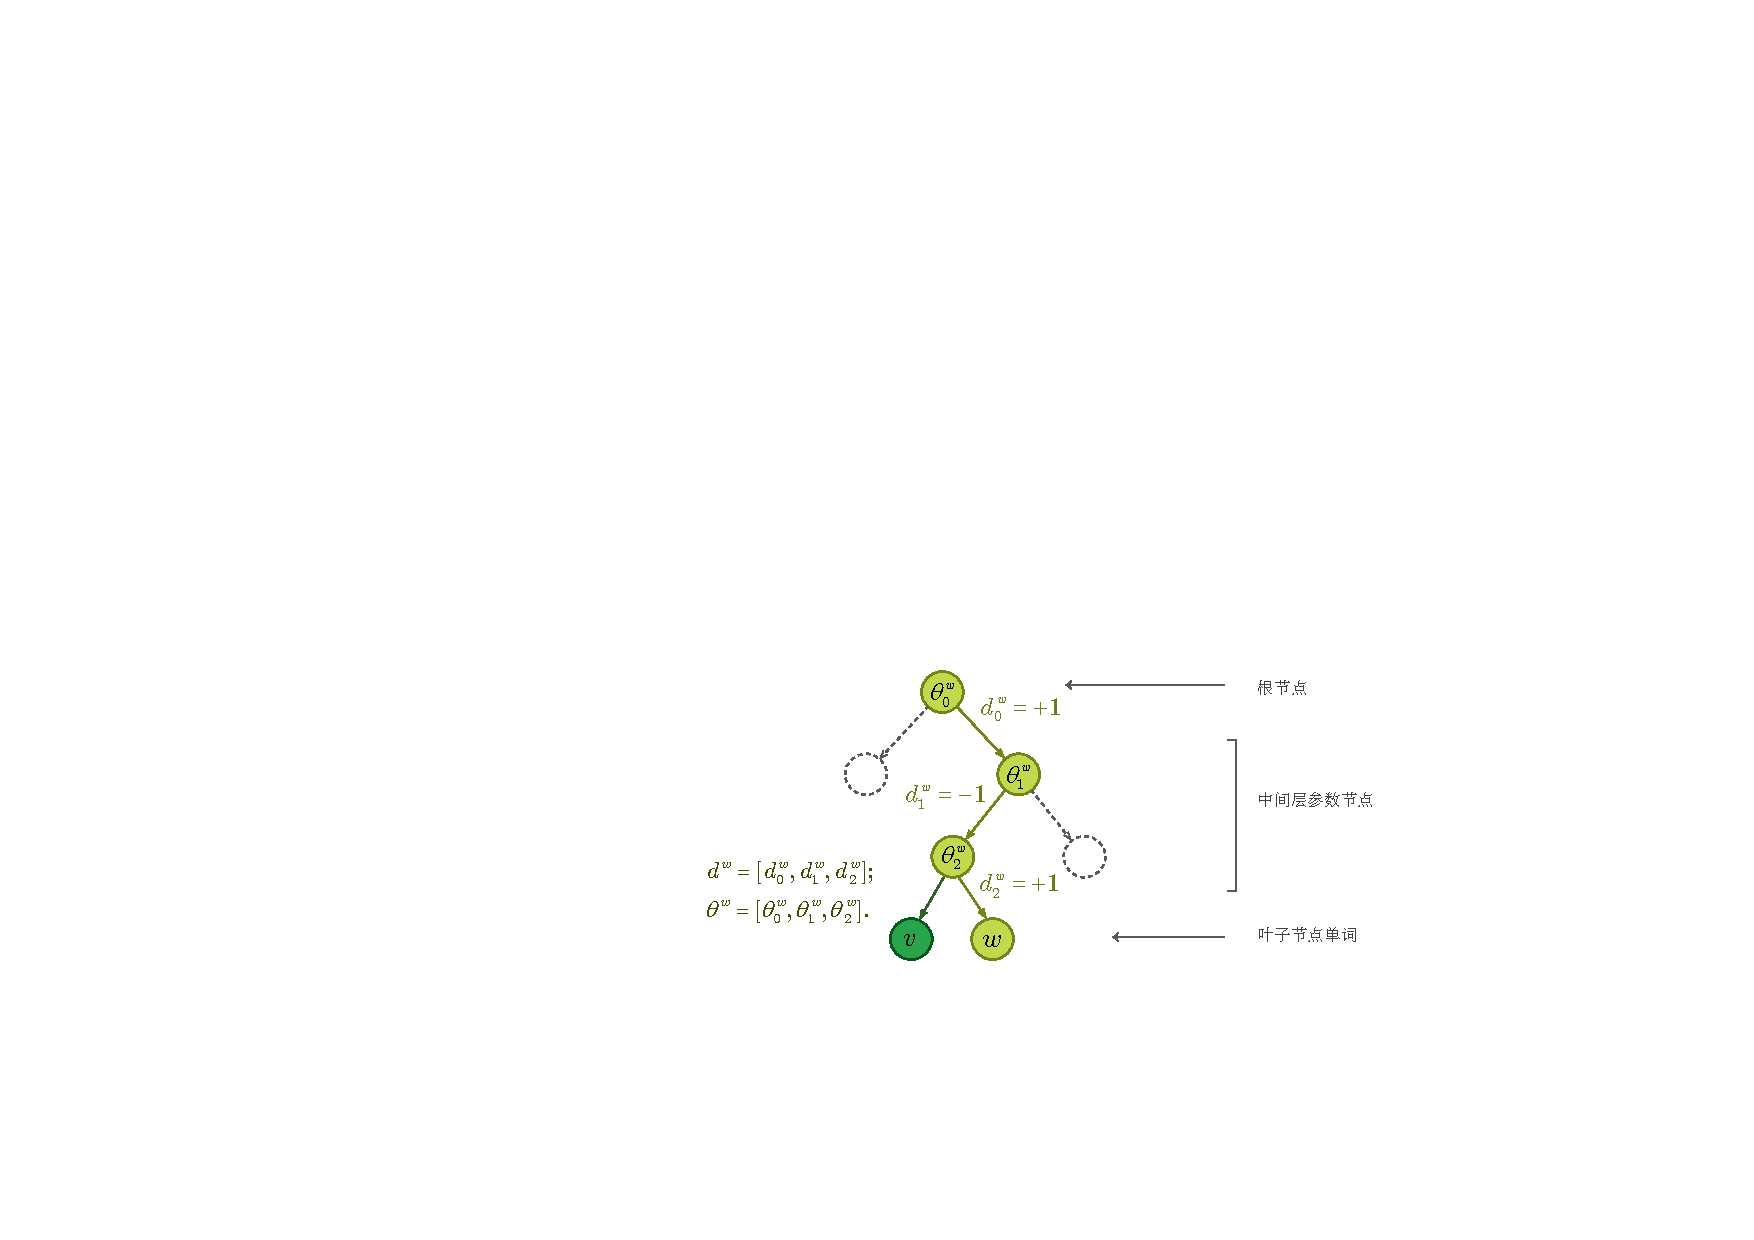
\includegraphics[width=0.75\linewidth]{./figures/thsm.pdf}
\caption{树状层次概率模型}\label{fig:tree_hsm} %
\end{figure}

\subsection{基于二叉树的代价函数和导数}
 \begin{equation}
p(d^w_i|\theta_{i}^w,h) =\sigma(\theta_{i}^w h)^{d_i^w}\times[1-\sigma(\theta_{i}^w h)]^{1-{d_i^w}},d_i^w \in [0,1]
\end{equation}
 \begin{equation}
p(d^w_i|\theta_{i}^w,h) =\sigma(\theta_{i}^w h)^{d_i^w}, d_i^w \in [-1,1]
\end{equation}
\begin{equation}
p(d^w_i=\pm 1|\theta_{i}^w,h) = \sigma({d_i^w}\theta_{i}^w h)
\end{equation}

一个单词的概率 $w$:
\begin{equation}\label{equ:pw}
\begin{split}
 \log p(w|h)=&\log\prod_{i=0}^{l^w-1} p(d^w_i|\theta_{i}^w,h) = \sum_{i=0}^{l^w -1} \log\sigma(d_i^w \theta_{i}^w h)\\
 =&\log\sigma({d^w}^\top \theta^w h)=\zeta(- {d^w}^\top \theta^w h )
 \end{split}
\end{equation}
其中 $\zeta(z)$ 代表 softplus 函数: $\zeta(z)= \log (1+\exp(z))$ 他的导数是 $\sigma$ 函数, 其导数公式是: ${\mathrm{d}\zeta(z)}/{\mathrm{d} z}= \sigma(z)$~\upcite{DBLP:conf/nips/DugasBBNG00}. Minimising the tree-based negative log-likelihood is directly maximising softplus loss and the probability of estimated words.

Nonetheless, in the traditional tHSM algorithm, the model calculates the log-probability of every node layer-by-layer. Consequently, the overall joint log-probability of this word is summarised linearly through the layers. Thus the time complexity of tHSM takes $O(\mathcal{|H|\log|V|})$:
\begin{equation}
\ell(\theta|h,w) =\sum_{i=0}^{l^w-1} \{(1-d'^w_i)\log (\sigma(\theta_{i}^w h))  + {d'^w_i}\log (1-\sigma (\theta_{i}^w h))\}
\end{equation}
where $d'^w_i\in \{0,1\}$, and these two parts model the joint probability distribution of the left and right branch of internal nodes separatively.

Noticeably, the main difference between p-tHSM and tHSM is that: a) tHSM algorithm involves many tiny matrix multiplications, instead in p-tHSM we load all parameters $(d^w, \theta^w)$ directly as 1D vector and 2D matrix at the expense of runtime memory consumption and we consider the multiplications of this vector and giant matrix, as shown in Fig.~\ref{fig:tree_hsm}; b) A compact loss function of the model is deducted and the nodes' log-probability are calculated simultaneously which results in better time efficiency for p-tHSM model.

As a consequence, the model's parameters $\{\theta^w,h\}$ are optimised with regard to its gradient.
\begin{equation}
\begin{split}
\frac{\partial \ell}{\partial \theta^w}=&(\sigma({d^w}^\top\theta^w h) -1){d^w}^\top h \\
\frac{\partial \ell}{\partial h}=&(\sigma({d^w}^\top \theta^w h) -1){d^w}^\top \theta
\end{split}
\end{equation}

\begin{figure}[!ht]
  \centering
\includegraphics[width=0.45\linewidth]{./figures/relus.pdf}
\caption{Softplus和ReLU函数的示意图}\label{fig:soft}
\end{figure}

二叉树分解的一个主要优点是它避免了在整个词汇表中概率的归一化,因为树中词的汇总概率自然等于1。
\begin{equation}
\sum_{w\in \mathcal{V}}{p(w|h)}=\sum_{w \in \mathcal{V}}\sum_{i=0}^{l^w-1}{\sigma(d_i^w\theta_{i}^w h)}=1.
\end{equation}




\subsection{基于二叉树的推理算法}
考虑到本节开始提出的第一个问题,即给定序列$ [w_1,\ cdots,w_T] $的概率。 直观地说,当给定相应的上下文$ h $时,我们可以通过获取一个特定单词$ w $的概率或对数概率来分解问题:
\begin{equation}
\begin{split}
    p(w|h) =&\sigma({d^w}^\top \theta^w h)\\
   \log p(w|h) =& -\zeta(- {d^{w}}^\top \theta^{w} h )
\end{split}
\end{equation}
其中概率$ p(w | h)$和单词$ w $的对数概率$ \log p(w | h)$可以直接通过等式~\ref{equ:pw}和~\ref{equ:cost}分开。 因此,这个序列的概率可以形式化为:
\begin{equation}
\ell(\theta|h,w) =\sum_{i=0}^{l^w-1} (1-d'^w_i)\log (\sigma(\theta_{i}^w h))  + {d'^w_i}\log (1-\sigma (\theta_{i}^w h))
\end{equation}
显然,这种类型的操作比传统的softmax方法有效得多,它涉及$\mathcal{O}(\mathcal {| H | \log| V |})$计算。

关于第二种情况,当给定前一个上下文(也被称为$\arg\max $方法)时,在整个词汇表中搜索最可能的下一个话语单词。我们可以在选择最上面的一个候选人之前计算词汇表中所有单词的概率。这个过程仍然是昂贵而缓慢的,因为它涉及到整个词的分层树。如在算法~\ref{alog:argmax}中所描述的,为了避免两个小概率的精确度损失问题,计算每个内部节点的对数概率。

而不是搜索全局最优结果,我们可以用局部贪婪算法搜索次优结果。具体而言,对于$ i $ -th层中的节点,当$ p(d ^ w_i | \theta_{i} ^ w,h)\ge 0.5 $时选择左边的分支,相反适用,如算法~\ref{alog:greed_argmax}所示。因此,计算时间复杂度仍然是$ \mathcal{O}(| H | \log \mathcal {| V |})$。


\begin{algorithm}[!ht]
\SetAlgoLined
\KwData{隐藏层输出 $h$;}
\KwResult{ 预测的单词 $w$. }
 路径列表 $\mathtt{path}$=[] \;
\While(\tcp*[h]{逐层搜索}){$k \le \log \mathcal{V}$ }{
\eIf{$p(d_{k} |\theta_{k},h) \ge 0.5$ }{
 $k=  k*2$ \tcp*[r]{左分支}
}{
 $k = k*2+1$ \tcp*[r]{右分支}
}
 $\mathtt{path}$.append($k$) \tcp*[r]{append $k$ to path list}
}
 alter $\mathtt{path}$ with word $w$ by looking-up table $\Gamma$.\
 \Return $w$ \;
\caption{逐层贪心搜索 Argmax}\label{alog:greed_argmax}
\end{algorithm}

\subsection{基于二叉树的聚类算法}
词汇表中每个单词$(d^w,\ theta^w)$的极性编码与树的结构密切相关。对于提出的p-tHSM方法,我们采用了几种树聚类算法来提高其性能和稳定性。这些聚类算法为每个单词生成二进制前缀字符串,表示树中单词的位置,并将用于初始化p-tHSM方法。


1)\textit{Unigram 聚类}它根据词频对词汇进行排序,并根据单词统计从buttom到top进行合并,也称为Huffman Encoding~\upcite{DBLP:conf/nips/MikolovSCCD13}。

2)\textit{Bigram 聚类\footnote{https://github.com/percyliang/brown-cluster}}。它是一个层次凝聚聚类算法,使用bigram上下文来确定单词的分布相似性,将相似的单词放置在二叉树的附近位置~\upcite{DBLP:journals/coling/BrownPdLM92,liang2005semi}。在将簇大小指定为1之后,它从底部到顶部合并具有一个节点的单词。生成的单词二进制路由正是分层二进制结构的分布。

3)\textit{语义聚类\footnote{https://code.google.com/archive/p/word2vec/}。}在引导式的方式下,词嵌入在外部语料库上训练,我们将传统的凝聚式聚类应用于字嵌入特征~\upcite{DBLP:books/sp/mining12}。

\section{模型二}
\subsection{词表划分算法}
为了提高GPU架构的加速比,并支持广义的词汇分割方法,我们提出了一种基于类的分层softmax方法的高效通用结构。

扁平化的词汇表被分成类别向量$ \theta^c $和输出矩阵$ \theta^o $ 结构,其中前者定义了不同类别的概率$ p ^ c $,而后者则模拟了该分区组内的单词概率$ p ^ o $,如图~\ref {fig:chsm}所示。输出矩阵的维度是类维度和分组词维度。如果将词汇$ \mathcal {V} $划分为不等大小的组,我们首先将词组分类为等长矩阵,填充零掩码。对于不在这个组中的剩余节点,我们使用掩码向量$ \ theta ^ m $来消除其对概率计算和成本汇总过程的影响。因此,分组的文字尺寸是最大的组尺寸。如果我们应用相同大小的词汇分割算法,掩码向量$ \theta ^ m $可以被忽略,并且分组的词维度是$ \mathcal {| V | / | C |} $,其中$ \mathcal {| C |} $表示类维度。要注意的是,如果$ \mathcal {| V |} $不能被$ \mathcal {| C |} $整除,那么最后一组中的确切单词应该小于组大小。

更重要的是,我们将一次性索引设置分成一个元组$(w ^ c,w ^ o)$,可以从查找表$\Gamma $中检索给定单词索引$ w $。此外,$ w ^ c $指定类ID,$ w^c $表示该组内的本地单词索引。
\begin{equation}\label{equ:partition}
 \theta^m=
\begin{cases}
    \text{单位矩阵} ,& \text{若均匀划分} \\
    \text{掩码矩阵},   & \text{否则}
\end{cases}
\end{equation}


如图~\ref{fig:chsm}~所示,扁平化的词汇可以形成右上矩阵,矩阵的大小应该大于或等于词汇表,不需要外部掩码。
另外,拼合词汇可以形成左上矩阵,需要外部掩模,矩阵的构成依赖于分割算法。
\begin{figure}[!ht]
  \centering
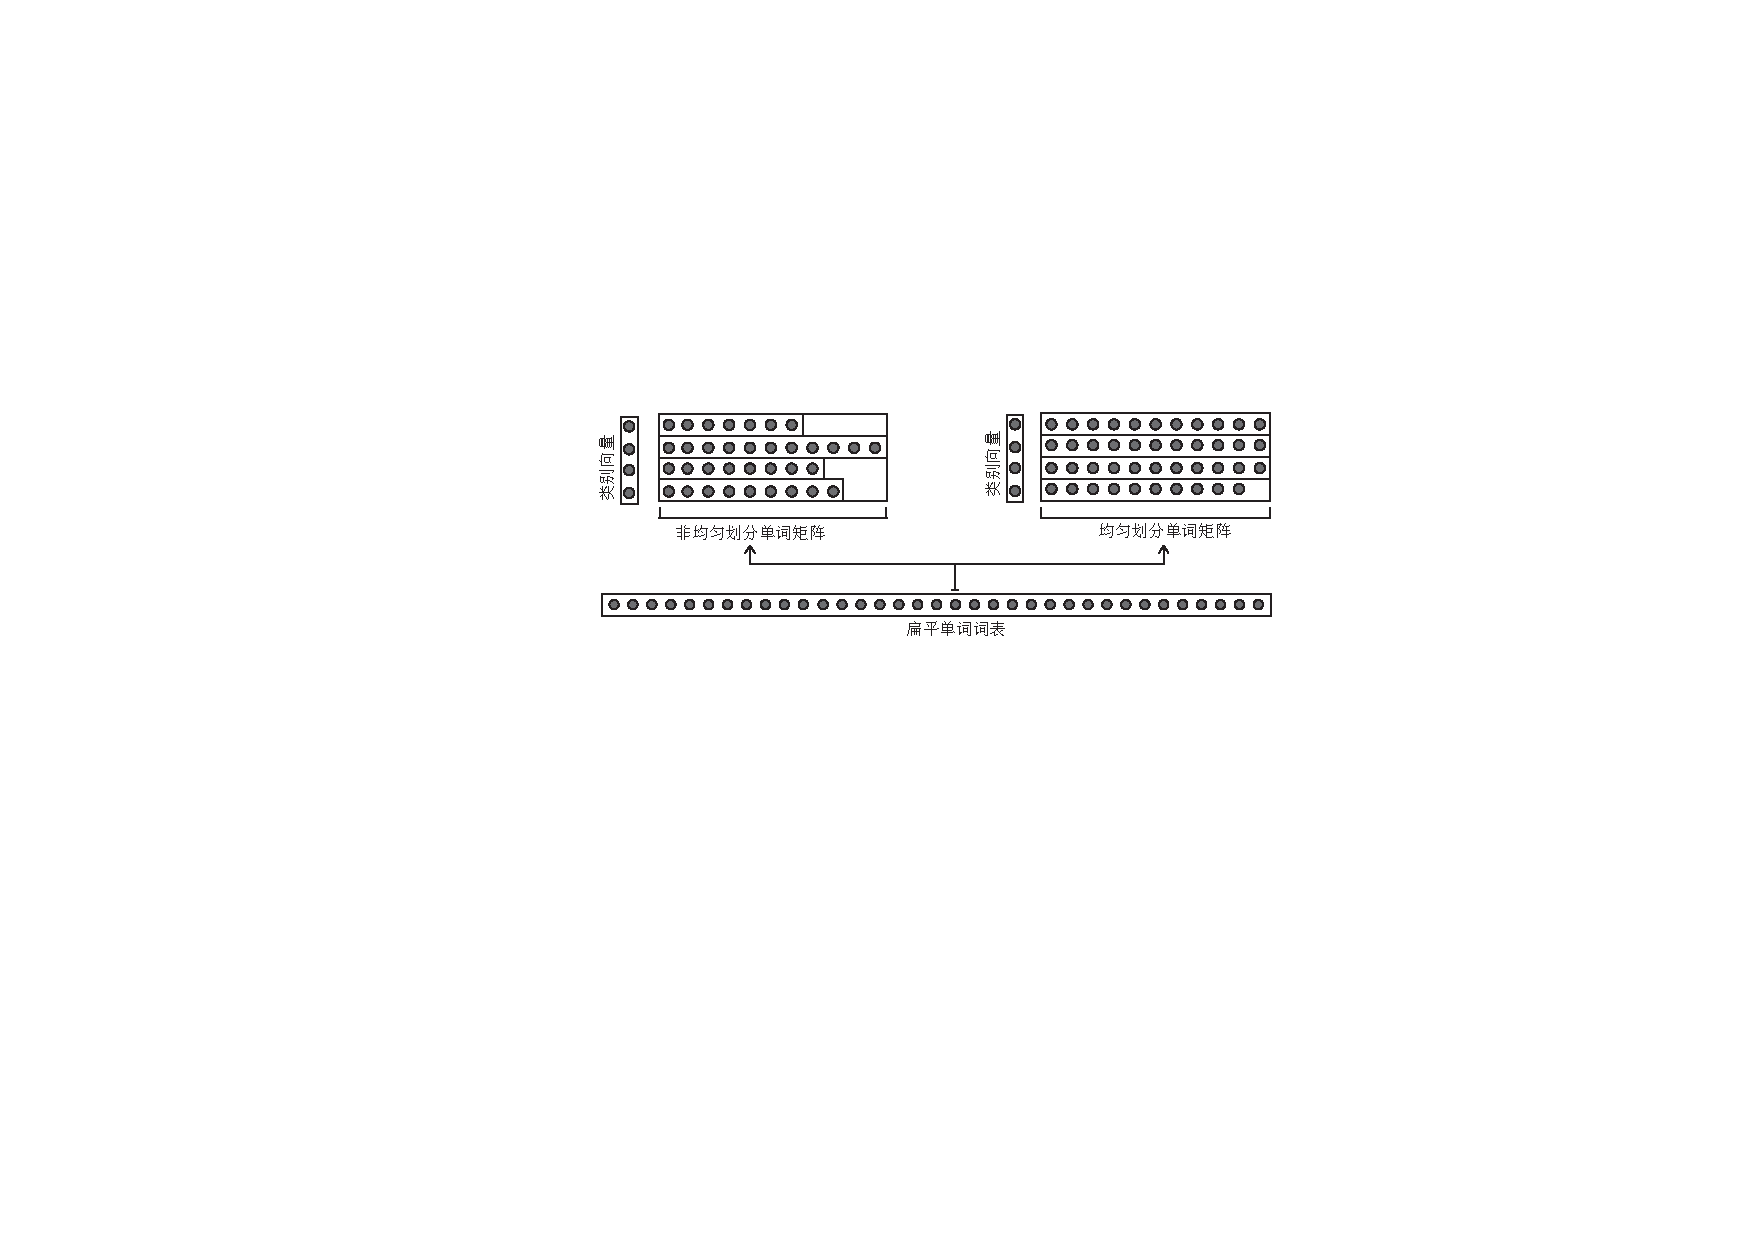
\includegraphics[width=0.85\linewidth]{./figures/chsm-simple.pdf}
\caption{cHSM算法的两种不同的词表划分算法}\label{fig:chsm}
\end{figure}


\subsection{基于类别的代价函数和导数}
给定最后一个隐藏层输出$ h $,那么这个分区组中的每个组和每个单词的概率可以被定义为:
\begin{equation}
\begin{split}
\log p^c(c|h) &= \theta^c h-\log \sum{\exp( \theta^c h )} \\
\log p^g(w|w^c,h)&=\theta^o h -\log\sum\exp{(\theta^o h)}
\end{split}
\end{equation}
其中$ p ^ c $和$ p ^ w $是分别计算而不是并行计算的,因为主要的计算瓶颈是局部标准化的单词概率$ p ^ w $,所以这两个概率的并行计算不会达到时间效率提升。


尽管如此,掩码矩阵不能直接应用于这个分词矩阵,应该应用在log softmax概率计算程序中。 为了说明,在softmax函数中:$ p(x_i)= {\exp({x_i}})/ {\sum_j \exp(x_j)} $,如果$ x_k = 0 $,但其概率$ p(x_k)> 0,\quad \exp(x_k)> 0 $。 因此,该组中确切的后验词对数概率计算如下:
\begin{equation}
  \log p^o(w|w^c,h)=\theta^o h -\log\sum\theta^m\exp(\theta^o h)
\end{equation}

那么,这个模型的损失函数可以形式化如下:
\begin{equation}
\ell(\theta|h) =\log p^c(w^c|h) +\log p^o(w^o|w^c,h)
\end{equation}
其中类别水平损失等于负对数似然的常见设置,并且字水平损失需要在计算其损失时指定其类别 $ w ^ c $。

在训练过程中,$ w ^ c $是预定义的,在测试过程中,$ w ^ c $由$ \arg\max_c p ^ c $获取。 类似地,关于梯度,模型的参数被优化。
\begin{equation}
\begin{split}
\frac{\partial \ell}{\partial \theta^c}=& (\delta_{ij}-p(c|h))h \\
\frac{\partial \ell}{\partial \theta^o}=&(\delta_{ij}-p(w|c,h))h \\
\frac{\partial \ell}{\partial h}=&(\delta_{ij}-p^c(c|h))\theta^c + (\delta_{ij}-p^o(w|c,h))\theta^o
\end{split}
\end{equation}

将词汇分成相互排斥的词组的一个主要优点是:a)避免了在整个词汇表上规范概率。 由于$ p ^ c $是在类维度上标准化的,$ p ^ o $是在最大组大小上进行标准化的。 所以在第二个方程中,多余的其他组被忽略,在最大的文本数据集中二者都不会超过1000。 b)与基于树的结构相比,它在词汇表上的分布更少,在分解步骤中丢失的信息更少。 c)与子字级方法相比,它不会增加序列长度,也不会影响复发性细胞的长程依赖性建模。



\subsection{基于类别的测试推理}
在推理阶段,对于cHSM模型来说,序列的概率评分要容易得多。
类似于以前的方法,我们可以通过重新研究我们的训练模型来解决第一个问题:
\begin{equation}\label{equ:class_inf}
   \log p(w_1,\cdots, w_T)=\sum_t^T\log p(w_t|h_t)=\sum_{t=1}^{T}\log p^c(w^c_t|h_t) +\log p^o(w^o_t|w^c_t,h_t)
\end{equation}
我们发现这种类型的操作比传统的softmax方法有效得多,该方法涉及$ \mathcal{O (| H | \sqrt{|V|} )}$计算。

其次,对于$\arg\max $的情况,我们可以在选择最佳候选项之前计算词汇表中所有单词的概率,这在直观上是正确的,但在计算上是昂贵的且慢,因为涉及到整个单词的分割矩阵。 此外,我们仍然可以在算法~\ref{alog:exact}~中对上述方法进行少量修改,然后计算确切的最高候选人。
\begin{algorithm}[!ht]
\caption{Exact $\arg\max$ algorithm for cHSM.}\label{alog:exact}
\KwData{ 隐藏层输出 $h$;}
\KwResult{ The predicted best candidate word $w$.}
 $\hat y^o=\arg\max_o{\log p^o(w| c,h)}$ \tcp*[r]{select best candidates in every group}
 $\tilde y^c=\arg\max_c{(\log p^c(y^c|h)+\log p^w(\hat y^w|\hat y^c,h))}$\tcp*[r]{calculate best candidate}
 alter $(\tilde y^c,\hat y^o[\tilde y^c])$ with word $w$ by looking-up table $\Gamma'$ \;
 \Return $w$ \;
\end{algorithm}

此外,cHSM算法的性能对分区算法有些敏感,因为某些方法可能会产生高度不平衡的字组,并且这种偏斜的分布会在算法中产生标签偏差问题。第一个本地 $\arg\max_o$ 进程~\upcite{DBLP:conf/icml/LaffertyMP01}。然而,在大多数情况下,如果选择合适的参数,则可以考虑不平衡的问题,本文考虑平衡词汇分区的广义形式。

为了说明,考虑两个类 $ c_p $ 和 $ c_q $,这两个类的容量是不同的,例如 $| c_p | \le | c_q |$。在计算了最后一个隐藏层输出 $h$与类图层参数的相似性之后,我们继续计算 $h$ 与每个组的内部单词 $w$ 的相似性得分,这些单词在每个特定组中都没有进行局部规范化整个词汇。当$ | c_p | \approx|c_q|$ 表示我们希望将词汇聚类成等大小的群组,而不是高度倾斜的群组分布时,可以减轻标签偏差问题,其中$ | c_p | \ll | c_q | $ 。更具体地说,对于分布不均的情况,对于类 $ c_q $中的单词来说这个概率被一大群单词稀释是不公平的,这样算法更有可能以较高的概率取出这个小组中的单词,放弃在其他大集团有更多的潜在的话。

我们可以用局部贪婪算法搜索次优结果,而不是搜索确切的全局最优结果,而是建议将这个$ \arg\max $进程分解为两个阶段:a)计算类概率,并剔除顶端一个$ \hat c $; b)计算该类别的单词概率$ \hat c $,并选择具有最高本地单词概率的单词。这个算法会给psudo最好的候选人,但是与原始算法~\ref{alog:exact}相比,它的运行速度要快得多。而且,由于分组词在本地进行归一化,标签偏差问题可以在一定程度上缓解。在实验研究中将讨论算法~\ref{alog:exact}和~\ref{alog:argmax}的详细不同性能。
\begin{algorithm}[!ht]
\KwData{隐藏层输出 $h$;}
\KwResult{ The predicted best candidate word $\hat w$.}
 $\hat w^c=\arg\max_c{\log p^c(c|h)}$ \tcp*[r]{select best candidate among classes}
 $\hat w^o=\arg\max_o{\log p^o(w|\hat w^c,h)}$\tcp*[r]{select best candidate in specific group}
 alter $(\hat w^c,\hat w^o)$ with word $\hat w$ by looking-up table $\Gamma'$ \;
 \Return $\hat w$
 \caption{Psudo $\arg\max$ algorithm for cHSM.}\label{alog:argmax}
\end{algorithm}

\subsection{词表划分算法}
由于cHSM模型的性能与其词汇分割算法密切相关,我们将聚类算法的现有工作进行汇总,并将可能的方法分类如下:

1)\textit{随机初始化} 这种直观的方法忽略了单词的所有外部信息,因此单词与随机随机播放过程是等分的。这是揭示其他聚类方法下界的最坏情况,也可以揭示应用高级聚类策略的相对收益。

2)\textit{字母顺序} 这种方法根据字符级别的信息对单词进行排序,同一组中的单词共享一个相似的子字符串。

3)\textit{Unigram 聚类}这些单词首先根据它们在文本中的频率排序,然后通过放置边界使得每个类别占总概率质量的恒定部分,从而形成连续单词块。这种方法具有这样的性质:较低编号的类比较高编号的类具有更少的成员,因为它们的成员更频繁~\upcite{DBLP:conf/nips/MikolovSCCD13}。

4)\textit{Bigram聚类}。它是指布朗聚类方法,这是历史适用于基于n-gram的基于类的模型~\upcite{DBLP:journals/coling/BrownPdLM92,liang2005semi}。单词使用相同的bigram上下文分组到相同的行中。

5)\textit{结构聚类\footnote{https://github.com/AlonDaks/unsupervised-authorial-clustering}。}根据文本中的词性和句法结构划分词汇~\upcite{daks2016unsupervised} 。

4)\textit{语义聚类。}我们将传统的kmeans聚类方法应用到预训练的词嵌入,使得我们可以通过指定聚类的大小将词汇分成不同的形状。
\section{本章小结}

\chapter{语言模型实验及实验结果分析}
在前面两章中,本文按照章节分别介绍本文中使用的方法具体过程。在本节中,为了验证所提出的分层softmax方法与其他基线方法的效率和准确性,我们在三个标准文本数据集(Wikitext-2,Wikitext-103和One Billion Word数据集)上进行了循环语言建模任务的实验研究。本文将会展示并行层次概率计算算法的实验结果,并且在第二小节中展现实验结果,以及与其他加速算法的对比。 此外,还从“效率分析,可扩展性,参数和性能基准”四个方面对这些方法进行了实证分析。

\section{实验设置}
如表~\ref{tab:dataset}所示,三个数据集的单词数量,句子数量,词表大小和OOV比例。
\begin{table}
  \centering
  \caption{WikiText-2, WikiText-103 和 One Billion Words 数据集统计指标。 \label{tab:dataset}}
\begin{tabular}{llrrrrr}
\toprule
数据集& 类型& 文章数 & 句子数量 &  单词数量 &词表大小 & OOV (\%) \\ \midrule
\multirow{3}{*}{Wikitext-2} &训练集& 600 & 36,718 & 2,088,628 & \multirow{3}{*}{33,278} & \multirow{3}{*}{2.6\%} \\
&验证集& 60 &3,760 & 217,646  & &\\
&测试集& 60 & 4,358 & 245,569 & &\\
\midrule
\multirow{3}{*}{Wikitext-103} &训练集& 28,475 &  1,801,350 &  103,227,021 & \multirow{3}{*}{267,735} & \multirow{3}{*}{0.4\%} \\
&验证集& 60 &3,760 & 217,646  & &\\
&测试集& 60 & 4,358 & 245,569 & &\\
\midrule
\multirow{3}{*}{One Billion Word} &训练集& --- &30,301,028&768,646,526&   \multirow{3}{*}{793,471} &   \multirow{3}{*}{0.28\%} \\
 &验证集& --- &  6,075 &   153,583 &&\\
 &测试集 & --- &  6,206 &   159,354 &&\\
\bottomrule
\end{tabular}
\end{table}
于Wikitext-2和Wikitext-103数据集,训练,验证和测试集自然是固定的,并且其词汇大小也已经被定义\footnote{https://metamind.io/research/the-wikitext-long-term-dependency-language-modeling-dataset/}。他们共享相同的有效和测试集,而Wikitext-103的训练集大得多。对于``One Billion Word''数据集\footnote{http://www.statmt.org/lm-benchmark/},我们将``./train/''目录中的所有数据视为训练集,选择第一和第二数据集作为相应的验证和测试集。这些数据集的详细统计数据在表格~\ref{tab:dataset}中进行了说明。


在将模型聚合到训练数据集上之后,针对语言模型的两个标准评估度量标准来针对不同的优化方法:\textit{Perplexity}($ \mathrm{PPL} $)和\textit{Word Error Rate}($\mathrm{WER} $)。为了说明,$ \mathrm{PPL} $是一个内在度量,代表了在候选人中选择下一个话语时的混乱程度。语言模型较低的困惑意味着在相同词汇下更好的可预测性。此外,在整个测试集上,平均负对数似然分是指数,表示我们直接优化了训练过程中的困惑度量。
\begin{equation}\label{equ:ppl}
   \mathrm{PPL}(w_1,\cdots,w_T)=\sqrt[T]{\frac{1}{\prod_{t=1}^T p(w_t|w_{1:t-1})}}
\end{equation}

此外,$\mathrm{WER}$是单词的萊文斯坦距離距离(一种类型的编辑距离),被定义为错误识别的单词(删除,插入,替换)占单词总数的百分比\footnote{https://martin-thoma.com/word-error-rate-calculation}:
\begin{equation}\label{equ:wer}
  \mathrm{WER} = \frac{\text{插入单词数 + 删除单词数 + 替换单词数}}{\text{全部单词数量}}
\end{equation}
除了以上的准确性度量,\textit{训练时间效率,词汇可伸缩性}和\textit{运行时内存消耗}也应该被视为衡量不同模型的重要指标。因此,我们分别从GPU和CPU的理论和经验角度分析了不同优化算法的评估指标。最后,进行实验并在三个标准文本数据集上收集结果。

在我们的实验研究中,每个使用Theano框架实现的模型都运行在一个独立的GPU设备上,它具有12GB的图形内存(即Nvidia K40m),允许使用大的嵌入矩阵乘法是可能的。然而,随着参数维数的增加,一个GPU显存资源被快速利用殆尽。

然后,对于wikitext-2数据集,最大序列长度固定为256,对于wikitext-103数据集,最大序列长度固定为100,对于10亿字数据集,最大序列长度固定为50,因为它需要更多的图形内存消耗。对于长度超过长度阈值的句子,修剪超出的尾部。由于我们测量的是语言模型的字级损失而不是序列级的分数,因此消除的字对模型训练的影响是有限的。另外,我们将Adam优化器应用于两个学习率(即$ lr = 0.06,0.001 $)设置。词汇因子分解方法应用较大,而传统的softmax和抽样方法应用较小的方法。

对于在WikiText-2数据集上运行的实验,我们在批处理大小为20的20个时期内运行,直到我们观察到验证集上的最小$ \mathrm{PPL} $。培训损失约4.8,最好的验证错误。而对于Wikitext-103数据集,在训练集上优化参数需要大约3-4个时间,因为训练集大约比较小的一个大50倍。此外,训练损失大约在5.1左右,为什么在 wikitext-2 数据集上更高的原因是我们预测的词汇量要大得多,所以混淆程度(即训练损失)应该更高。虽然我们发现模型可以很容易地收敛到局部最小点,验证误差在这个局部最小值的范围内振荡,但是Wikitext-2和Wikitext-103的唯一区别是训练数据的大小,表示收集很多训练数据不能保证模型在相同的验证和测试集上学得更好,而不是更普遍的结果。

此外,在“十亿字”数据集上运行实验相当具有挑战性,因为它需要更大的参数来拟合。所以我们应用优化的CUDA实现的RNN模型~\upcite{DBLP:journals/corr/AppleyardKB16},将RNN小区的计算时间降到最低。然而,等待模型收敛到训练集上需要480小时,因此我们可以在验证集上得到可能的结果。

\section{层次化词表比较}
我们首先介绍语言模型中每个模块的时间消耗,如图1所示。 我们计算运行不同的RNN小区及其梯度(即,RNN Grad)所需的时间,以及Wikitext-103数据集的大词汇表上的常规softmax,这与词汇表的常见大小相当。 我们用Theano框架和CUDA实现了RNN单元,其中RNN的运行时间可以缩短到极限。 从图中可以看出,使用优化的CUDA,softmax模块的影响比RNN单元及其梯度更重要,这就需要我们详细讨论softmax优化。
\begin{figure}[!ht]
%\setlength{\abovecaptionskip}{0pt}
%\setlength{\belowcaptionskip}{0pt}
  \centering
  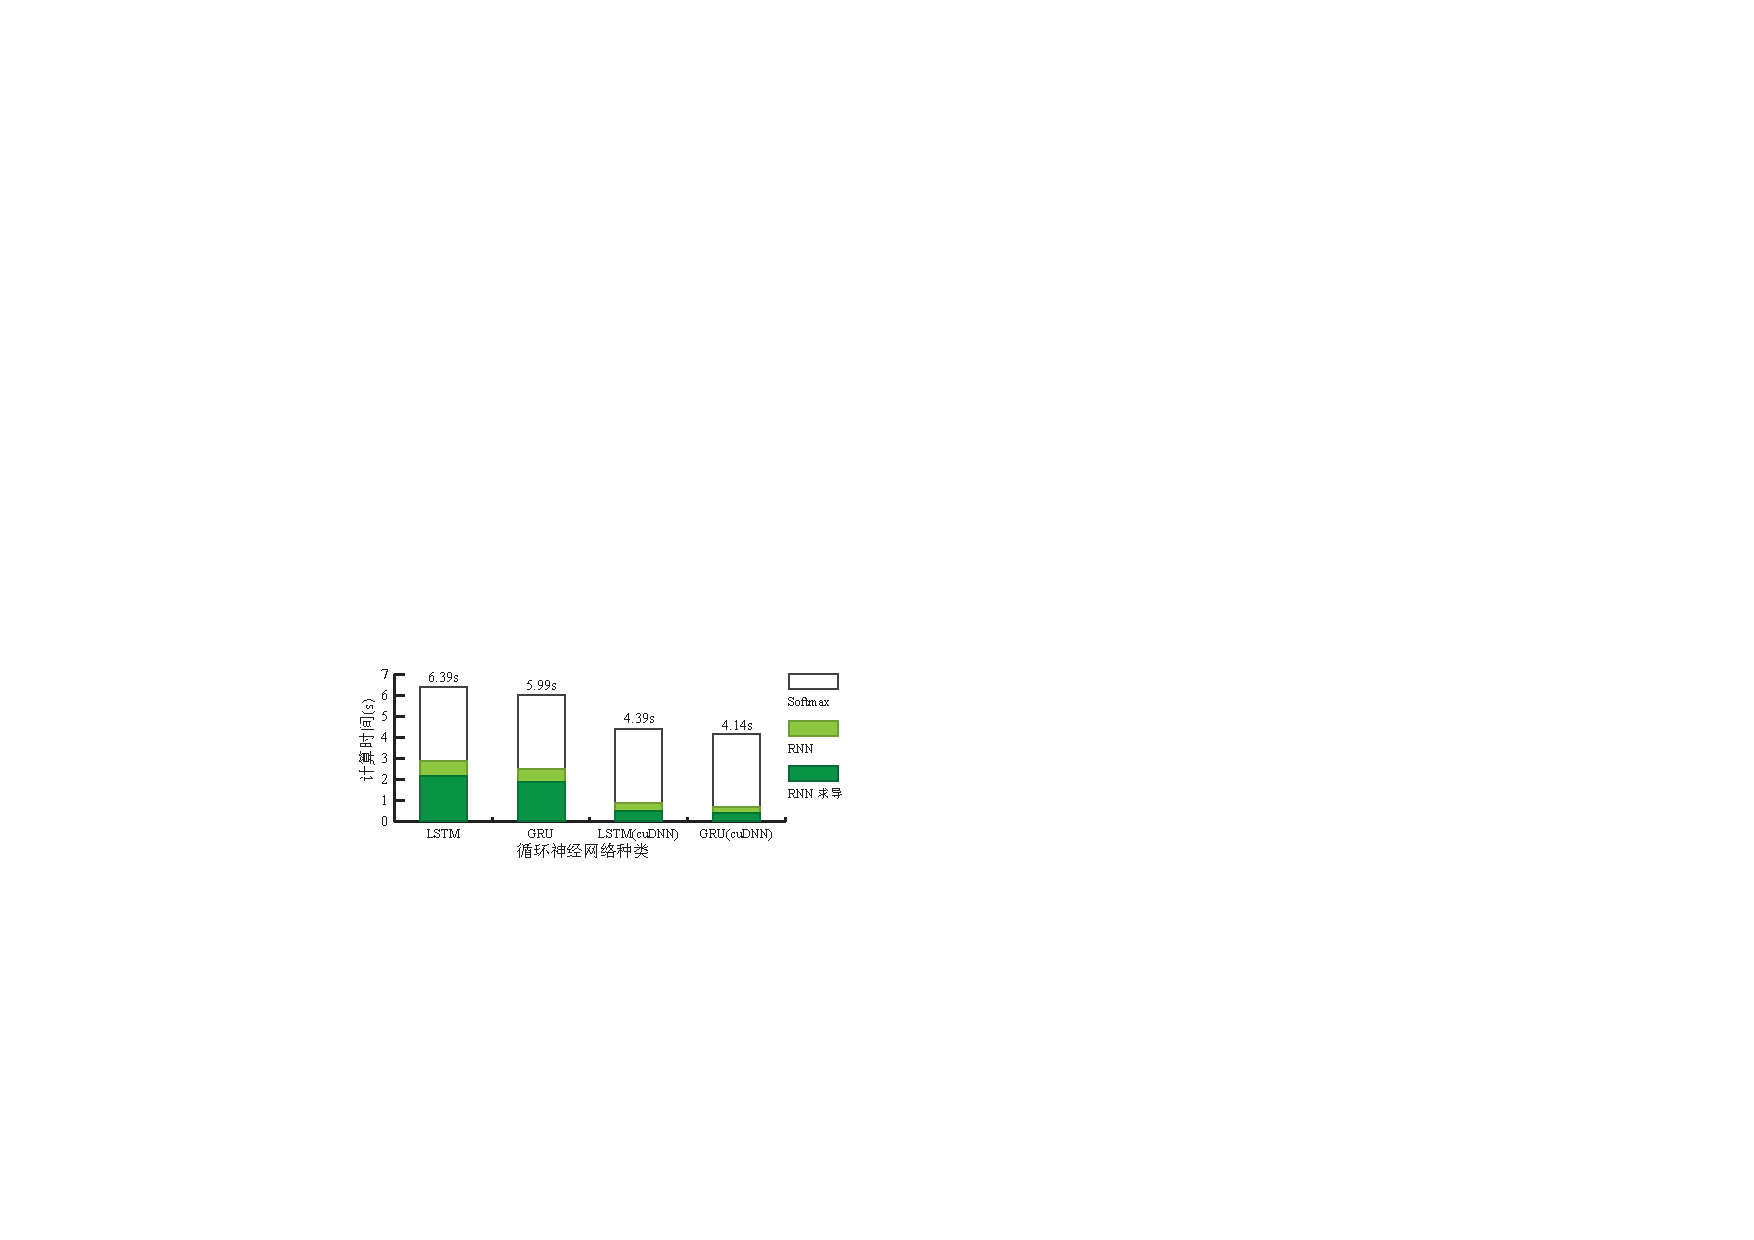
\includegraphics[width=0.6\columnwidth]{./figures/rnn_timing.pdf}
  \caption{Calculation Time of three modules with different recurrent cells on the Wikitext-103 dataset.}\label{fig:rnn_timing}
\end{figure}
\begin{figure}[!ht]
%\setlength{\abovecaptionskip}{0pt}
%\setlength{\belowcaptionskip}{0pt}
  \centering
  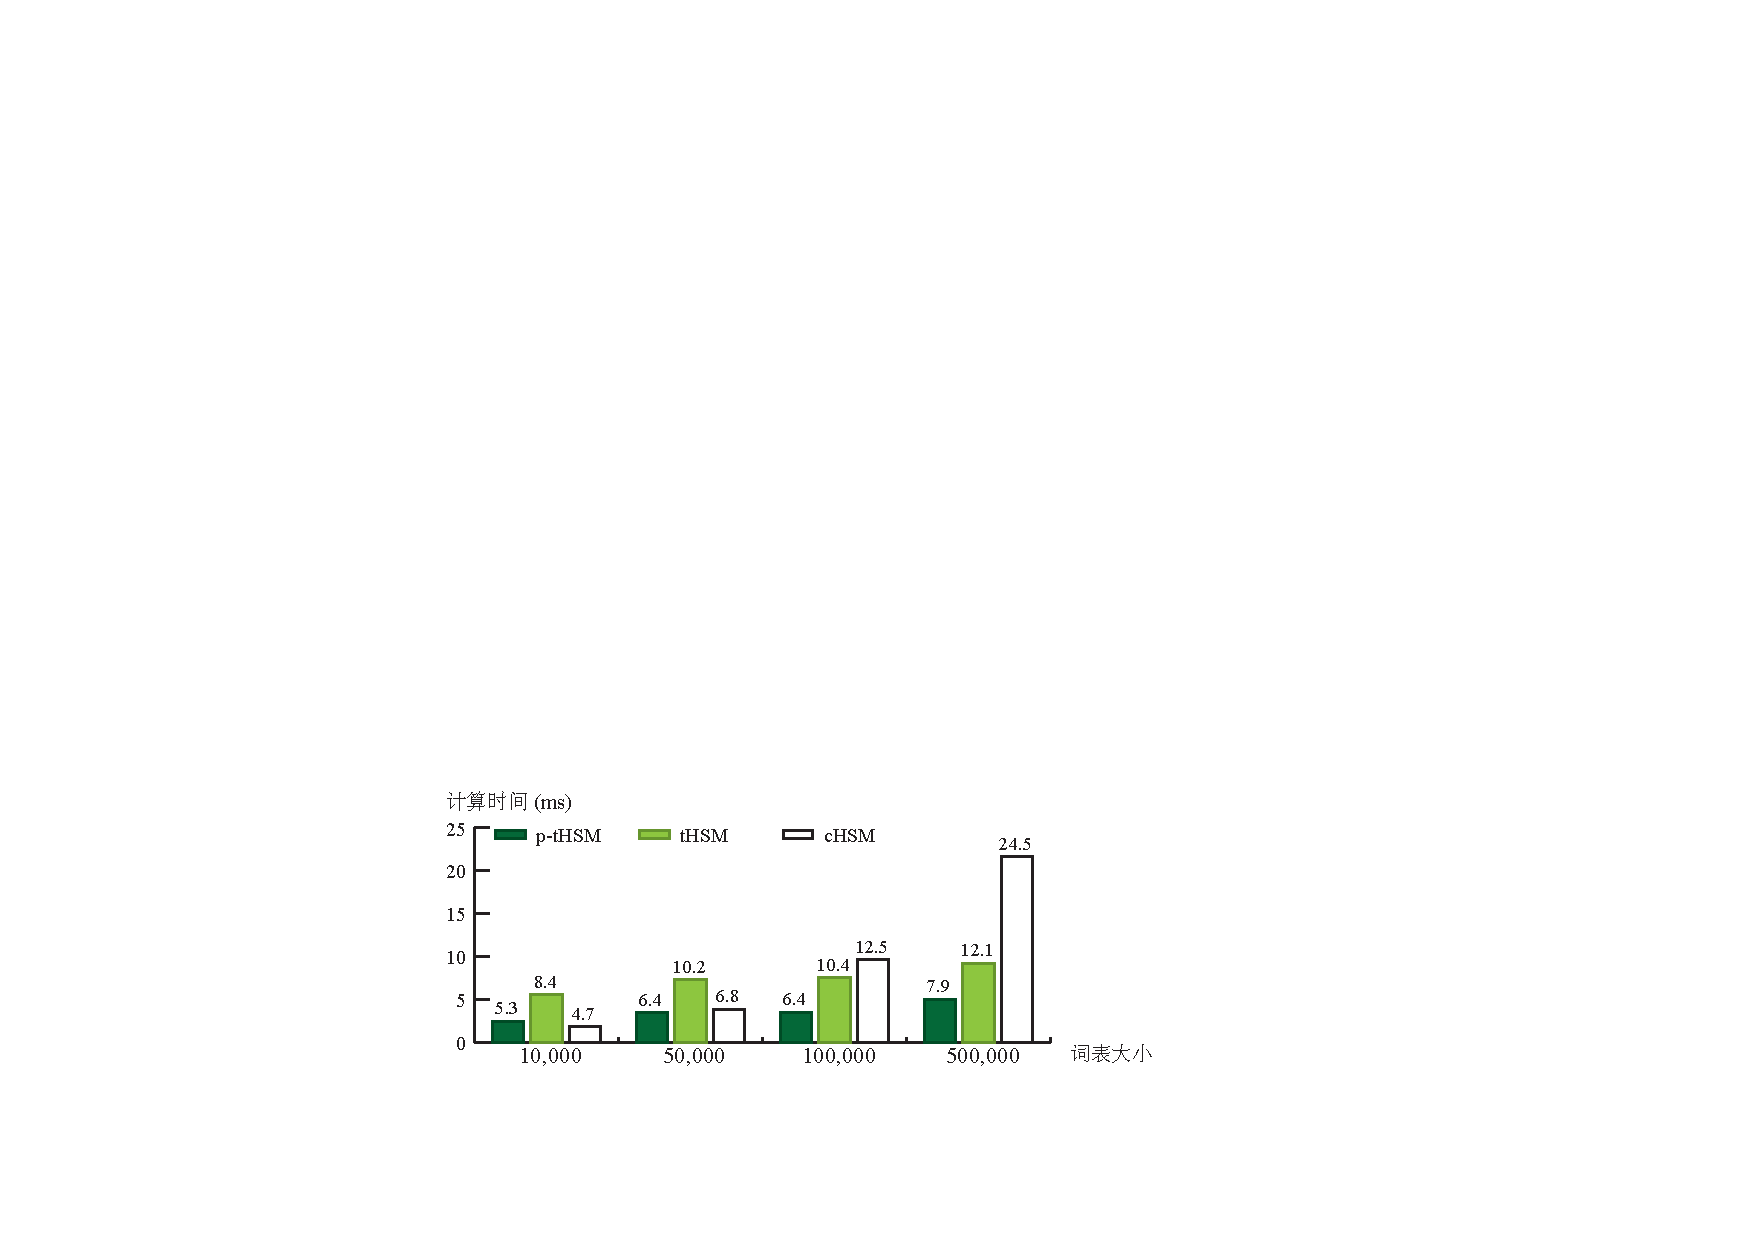
\includegraphics[width=0.6\columnwidth]{./figures/all_time.pdf}
  \caption{Scalability of cHSM, tHSM and p-tHSM algorithms with relevance to the vocabulary size.}\label{fig:hsm_benchmark}
\end{figure}
\begin{table}[!ht]
  \centering
  \caption{Runtime time and memory comparison on GPUs and CPUs with WikiText-103 Dataset.\label{tab:time}}
\begin{tabular}{lccccc}
  \toprule
 \multirow{2}{*}{算法}  &\multirow{2}{*}{运行时内存占用} &\multicolumn{2}{c}{总计算时间 (ms)} & \multicolumn{2}{c}{前向计算时间 (ms)}   \\
   \cmidrule(lr){3-4}  \cmidrule(lr){5-6}
	& & CPU&GPU & CPU& GPU \\ \midrule
Softmax & $\mathcal{|HV|}$ &510.4  &262.1&352.2& 62.9 \\
cHSM    & $2\mathcal{|H|\sqrt{|V|}}$&506.5  &\textbf{40.6}&28.7&14.6 \\
tHSM    &$\mathcal{|H|}$&1,004.0 &444.4 & 8.1&  5.6   \\
p-tHSM  &$\mathcal{|H|\log{|V|}}$ &\textbf{383.5}&	86.4 &\textbf{7.0}&	\textbf{1.4} \\
  \bottomrule
\end{tabular}
\end{table}


为了对用于训练相同批处理数据的经验时间复杂性和内存消耗进行基准测试,我们使用这些算法在表格~\ref{tab:time}中收集了GPU和CPU上的详细结果。我们尝试使用这些算法处理WikiText-103数据集,并计算处理一个批处理数据所需的平均时间。另外,输入句子的最大长度,隐藏层,输出词汇和批量大小分别设置为$\{50, 256, 267735, 20\}$。此外,“总时间”过程表示前向传播和后向梯度优化的过程,“前进时间”过程表示从输入数据到计算模型成本所需的时间消耗。此外,我们计算了上述算法训练期间加载所需的内存。 $ \mathcal{| V |} $表示词汇大小,$ \mathcal{| H |} $是目标嵌入维度。在训练期间,tHSM只消耗最小的存储器资源,而p-tHSM覆盖了更大的存储器集合,并且p-tHSM在考虑存储器消耗和速度时采用更大的存储器并且获得了更好的加速比。


\begin{table}[t]
%\setlength{\abovecaptionskip}{0pt}
%\setlength{\abovedisplayskip}{0pt}
  \centering
   \caption{Perplexity of p-HSM algorithms with various clustering methods on Wikitext-2 Dataset.\label{table:p-thsm}}
  \begin{tabular}{lcccc} \toprule
  Methods   &Build Time&Max Tree Depth &Validation Set (PPL) & Testing Set (PPL)  \\ \midrule
  Uigram  &3min&12 &218.42& 216.05     \\
  Bigram  &35h&21& 186.23& 189.58\\
  Semantic &26h &18& \textbf{163.12} & \textbf{178.78}\\
\bottomrule
  \end{tabular}
\end{table}

为了验证与词汇大小相关的cHSM,tHSM和p-tHSM算法的可扩展性,结果在图1中被收集。 为了显示p-tHSM算法的影响,不包含“Softmax”方法,因为与其他算法相比,它消耗了更多的计算时间。 很显然,cHSM随着词汇大小的平方根(即,$ \mathcal{O(| H | \sqrt{| V |})} $)进行缩放,而p-tHSM随着词汇大小的增加呈现出稳定的表现。

在这些实验的基础上,我们可以得出结论:所提出的p-tHSM方法胜过历史记录$ \mathcal{O(| H | \log| V |)})$,并且取得了令人满意的分层softmax方法的加速比。 这种性能归因于基于GPU并行性的加速,也是由于p-tHSM方法的基本结构,其将目标字树并行地维持。

\subsection{单词聚类策略分析}
陈等人发现cHSM的性能对~\upcite{DBLP:conf/acl/ChenGA16}这个词的聚类很敏感。同样,为了稳定cHSM和p-HSM方法的性能,我们考虑了几个现有的聚类准则,如表1和表2所示。

\begin{table}[t]
%\setlength{\abovecaptionskip}{0pt}
%\setlength{\abovedisplayskip}{0pt}
  \centering
  \caption{在Wikitext-2数据集上,cHSM 算法采用不同聚类算法的PPL 和 WER 结果 .\label{table:clustering}}
  \begin{tabular}{lclccc} \toprule
聚类算法 & 均匀划分?&分支数& 训练轮数& 测试集 (PPL / WER)&耗时 (ms)\\ \midrule
  \multirow{6}{*}{Random}  &\multirow{6}{*}{是}&10/3330&145&211.15 / 78.55 &791\\
    &&20/1664&123&228.72 / 78.89&565\\
    &&40/832&103&234.36 / 79.21&321\\
    &&80/417&78&243.12 / 79.64&171\\
    &&160/208 &57&253.38 / 80.08&92\\
    &&182/183&48&268.63 / 80.11&88\\
  \midrule
  \multirow{6}{*}{Alphabet}  &\multirow{6}{*}{是}&10/3330 &141&199.01 / 78.07 &773\\
    &&20/1664 &120&211.34 / 78.23&551\\
    &&40/832 &100&238.75 / 79.02&313\\
    &&80/417 &90&241.75 / 79.34&174\\
    &&160/208 &56&248.35 / 79.62&97\\
    &&182/183&45&258.57 / 80.02&87\\
  \midrule
  \multirow{6}{*}{Unigram}   &\multirow{6}{*}{是} &10/3330&134&211.51 / 77.41 &788\\
    & &20/1664&122&220.01 / 77.71&549\\
    & &40/832&113&236.56 / 77.95&302\\
    & &80/417&91& 241.12 / 78.25&170\\
    & &160/208&55&247.25 / 79.21&93\\
    & &182/183&42&253.35 / 79.92&86\\
  \midrule
  \multirow{5}{*}{Bigram}   &\multirow{5}{*}{否}&10/3672&150&208.11 / 77.32&801\\
     &&20/1923&121&217,34 / 77.64&621\\
     &&40/1123&102&228.87 / 78.14&588\\
     &&80/572&89&246.32 / 78.43&186\\
     &&160/340&76&252.33 / 79.51&97\\
  \midrule
  \multirow{5}{*}{Syntactic}  &\multirow{5}{*}{否}&10/3612 &152&214.31 / 78.11&810\\
    &&20/1972 &130&220.19 / 78.86&633\\
    &&40/996 &101&232.33 / 79.33&543\\
    &&80/545 &89&241.34 / 79.84&179\\
    &&160/235 &70&262.34 / 80.14&134\\
  \midrule
  \multirow{5}{*}{Semantic}  &\multirow{5}{*}{否} &10/3570 &133&208.77 / 77.41&819\\
    & &20/1873 &114&218.31 / 77.78&641\\
    & &40/1092 &91&225.38 / 78.35&521\\
    & &80/561 &69&238.45 / 78.91&174\\
    & &160/244 &44&256.75 / 79.41&103\\
\bottomrule
  \end{tabular}
\end{table}

一方面,我们将表~\ref{table:clustering}中的Wikitext-2数据集中的所有前面提到的聚类方法与不同的分支因子进行了比较。从这张表中可以发现,随机洗牌方法对于其他算法的性能最差,因为它们没有提供有关先前分配的任何信息。此外,还观察到,比其他人更难以接受可接受的训练损失,因此在训练集上花费更多的时间来优化参数。然后,发现在对类结构注入外部单字和双字的知识之后,模型确实在目标空间中学习了一个明确定义的单词分布。因此,它对随机和字母表系列取得了更好的结果。而且,用语法和语义算法进行分词的词汇比上述方法得到的结果要好得多,代价是计算分割方法。从实验结果可以看出,向具有先验知识的类结构注入会增强该方法的稳定性,通过平衡聚类时间和模型的准确性,可以调整分支因子,达到预期的结果。



另一方面,我们采用了单词,双字母和词汇聚类方法来生成单词在树上的分布,详细的结果在表格中给出。与提供调整分支因子的自由度的cHSM方法不同,树聚类的实验是相当有限的。单字聚类(即频率合并)方法在创建单词层次结构方面效率更高,而双字词和语义聚类花费更多时间来计算词汇表中单词之间的相似度矩阵。尽管如此,考虑到树合并的规则,bigram方法考虑了二元共现统计和语义方法来评估特征空间中的欧氏距离。在困惑度量下,二元语义聚类方法比一元方法有更好的效果。最后,与cHSM方法相比,更深层次的树模型更适合于词汇聚类,适当的聚类可以提高树层次的效率。

\subsection{搜索策略的影响}
由于我们提出了三个关于推理阶段搜索策略的算法,其影响可以通过WER度量来观察。在这个结构化预测过程中,一个合适的搜索规则将帮助模型获得最小风险的最佳候选人,如Table~\ref{tab:search}所示。 “全球”方法表示我们计算所有单词的得分,单词的概率用整个词汇全局归一化。值得注意的是,对于cHSM方法算法~\ref{alog:argmax}比算法~\ref{alog:exact}得到更好的WER,尽管后一种方法获得了词汇表上的确切顶级候选。由于类结构中存在标签偏差问题,排名最高的词容易出现算法模型无法建模的小组。最后但并非最不重要的是,算法~\ref{alog:exact}和``global''获得相同的单词排序,唯一的区别是算法~\ref{alog:exact}避免了冗余计算。所以他们达到了可比的WER得分,但算法~\ref{alog:exact}需要更少的时间。

对于p-tHSM系列,我们比较了所提出的算法~\ref{alog:greed_argmax}和传统的“全局”算法。算法~\ref{alog:greed_argmax}比“global”方法获得本地最佳结果花费的时间更少。由于基于树的模型在以前的决策中更容易失败,所以“全局”方法的MER分数要比算法~\ref{alog:greed_argmax}要好。

\begin{table}[!ht]
  \centering
  \caption{Word error rate with different searching rules on Wikitext-2 dataset.\label{tab:search}}
\begin{tabular}{llccc}
  \toprule
   & Type&Time (ms)&Validation set (WER)& Testing set (WER)\\ \midrule
  \multirow{3}{*}{cHSM} &global&102& 80.00\%& 80.02\%\\
        &Algorithm~\ref{alog:exact}&63& 80.00\%& 80.02\%\\
        &Algorithm~\ref{alog:argmax}&\textbf{44}&\textbf{ 77.09\%}&\textbf{ 77.07\%}\\\midrule \midrule
        & Type&Time (ms)&Validation set (WER)& Testing set (WER)\\ \midrule
  \multirow{2}{*}{p-tHSM}  &global&161& \textbf{76.67\%}&\textbf{75.35\%}\\
        &Algorithm~\ref{alog:greed_argmax}&\textbf{30} & 79.61\%&79.32\%\\
  \bottomrule
\end{tabular}
\end{table}

\subsection{Impact of Recurrent Cells}
\begin{table}[!t]
%\setlength{\abovecaptionskip}{0pt}
%\setlength{\abovedisplayskip}{0pt}
  \centering
  \caption{Results of different recurrent cells on Wikitext-2 dataset with metrics: PPL, WER and calculation time.\label{tab:rnn}}
\begin{tabular}{lccc}
  \toprule
  \multirow{2}{*}{Recurrent Cells} & \multirow{2}{*}{Time (ms)}&Validation Set & Testing Set\\
  && PPL / WER & PPL / WER\\ \midrule
  1$\times$RNN Relu~\upcite{DBLP:journals/jmlr/GutmannH10} &176.4&260.52 / 80.00\%&238.75 / 80.02\%\\
  1$\times$RNN Tanh~\upcite{DBLP:journals/iclr/JiVSAD15}   &176.2&250.57 / 79.61\%&230.98 / 79.32\%\\
  1$\times$LSTM~\upcite{7508408}                  &\textbf{189.5}&180.98 / 77.16\%&165.60 / 76.67\%\\
  1$\times$GRU~\upcite{DBLP:journals/corr/ChungGCB14}      &191.3&\textbf{179.59 / 77.09\%}&\textbf{165.32 / 77.07\%}\\ \midrule
  2$\times$RNN Relu~\upcite{DBLP:journals/jmlr/GutmannH10} &266.3&190.52 / 73.01\%&198.75 / 73.02\%\\
  2$\times$RNN Tanh~\upcite{DBLP:journals/iclr/JiVSAD15}   &266.3&189.57 / 72.62\%&260.98 / 72.32\%\\
  2$\times$LSTM~\upcite{7508408}                  &\textbf{279.4}&164.98 / 71.17\%&165.60 / 71.67\%\\
  2$\times$GRU~\upcite{DBLP:journals/corr/ChungGCB14}      &281.2&\textbf{158.59 / 70.08\%}&\textbf{155.32 / 70.07\%}\\
  \bottomrule
\end{tabular}
\end{table}

\begin{figure}[!ht]
%\setlength{\abovecaptionskip}{0pt}
%\setlength{\belowcaptionskip}{0pt}
  \centering
  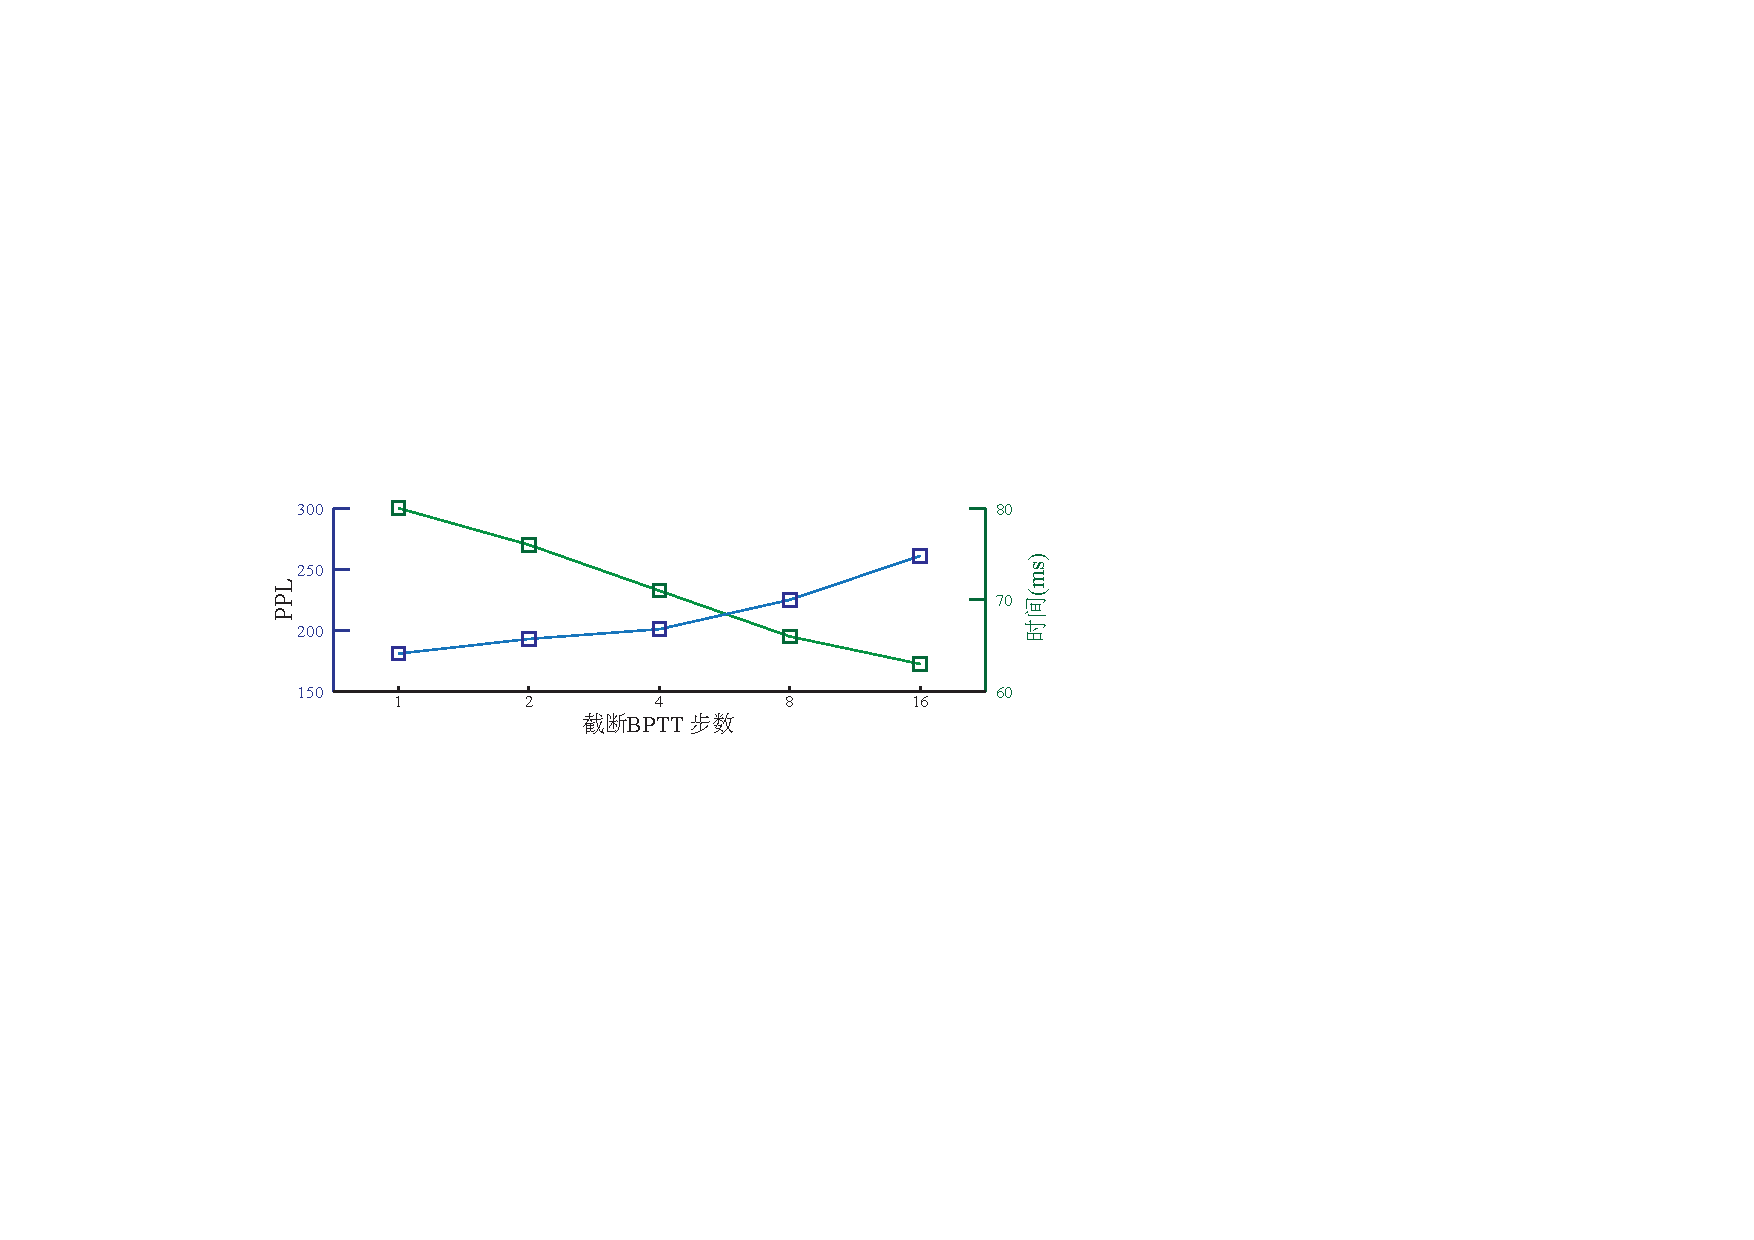
\includegraphics[width=0.65\columnwidth]{./figures/tbptt.pdf}
  \caption{Perplexity comparison of different Truncated BPTT Steps with the NCE and Blackout methods on Wikitext-2 dataset.}\label{fig:tbptt}
\end{figure}

\begin{figure}[!ht]
%\setlength{\abovecaptionskip}{0pt}
%\setlength{\belowcaptionskip}{0pt}
  \centering
  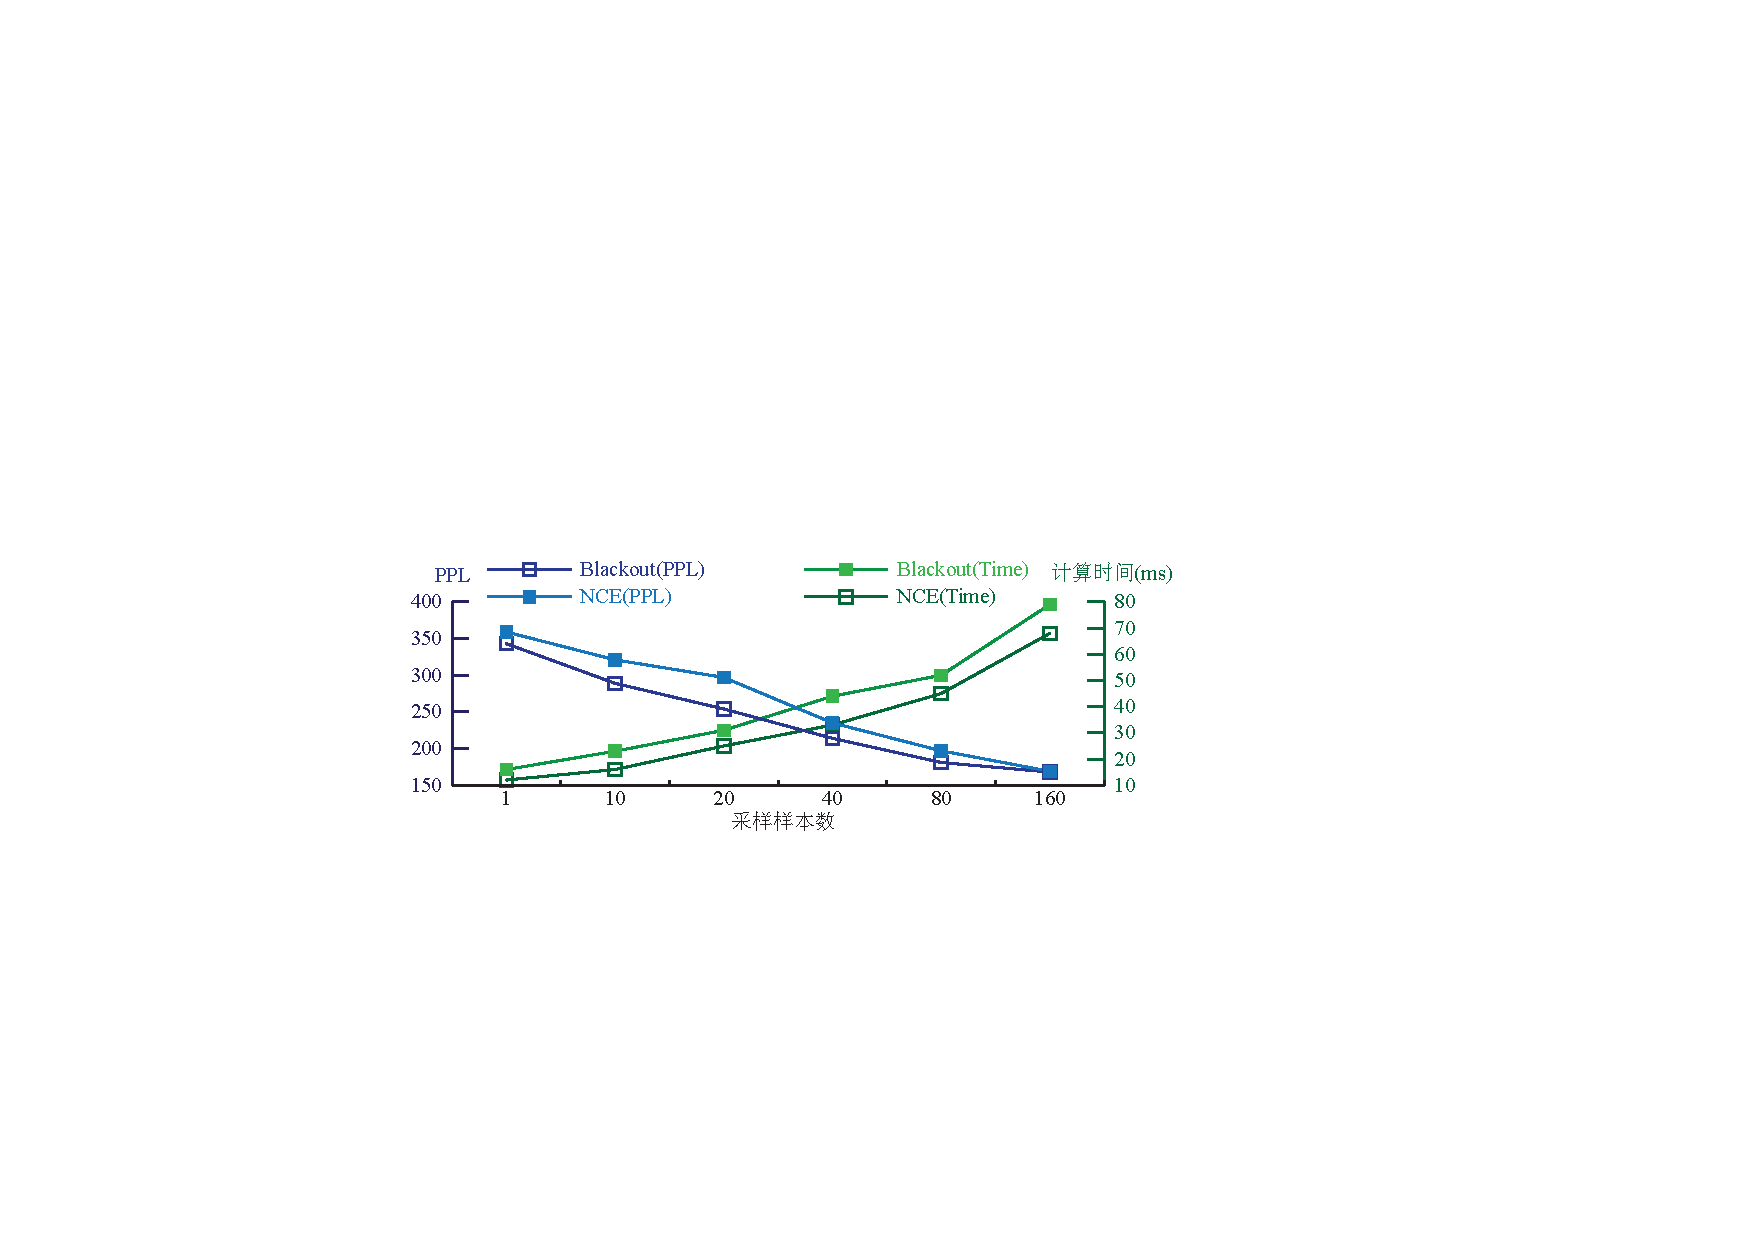
\includegraphics[width=0.65\columnwidth]{./figures/nce_blackout.pdf}
  \caption{Perplexity and time comparison of different sample size with the NCE and Blackout methods on Wikitext-2 dataset.}\label{fig:blackout_nce}
\end{figure}


\subsection{All Experiments Benchmark}

\begin{table}[!ht]
%\setlength{\abovecaptionskip}{0pt}
%\setlength{\abovedisplayskip}{0pt}
  \centering
  \caption{Perplexity and Word Error Rate on Wikitext-2,  WikiText-103 and One Billion Word Datasets.\label{tab:summary_ppl}}
\begin{tabular}{llcc}
  \toprule
数据集& 算法& 验证集(PPL/ WER) & 测试集(PPL/WER) \\ \midrule
 \multirow{2}{*}{WikiText-2}&GRU + Softmax&172.64 / 77.49\%&162.09 / 77.07\% \\
  &GRU + NCE~\upcite{DBLP:journals/jmlr/GutmannH10}&217.84 / 78.26\%&199.54 / 78.02\%\\
  &GRU + Blackout~\upcite{DBLP:journals/iclr/JiVSAD15}&221.15 / 77.72\%&199.56 / 77.50\% \\
  &GRU + cHSM + unigram~\upcite{DBLP:conf/acl/ChenGA16}&253.18 / 78.25\%&236.61 / 78.02\%\\
  &GRU + p-tHSM + unigram~\upcite{DBLP:conf/nips/MikolovSCCD13}&218.42 / 78.15\%&216.05 / 78.15\%\\
  &GRU + p-tHSM + bigram~\upcite{DBLP:journals/coling/BrownPdLM92}&186.23 / 78.15\%&189.58 / 78.15\%\\\midrule
   \multirow{2}{*}{WikiText-103} &GRU + Softmax&130.38 / 72.15\%&136.83 / 72.37\%\\
 &GRU + NCE~\upcite{DBLP:journals/jmlr/GutmannH10}&164.78 / 73.22\%&165.01 / 73.34\%\\
  &GRU + Blackout~\upcite{DBLP:journals/iclr/JiVSAD15}&163.99 / 73.18\%&162.76 / 74.22\%\\
  &GRU + cHSM + unigram~\upcite{DBLP:conf/acl/ChenGA16}&171.81 / 73.42\%&166.74 / 73.18\%\\
  &GRU + p-tHSM + unigram~\upcite{DBLP:conf/nips/MikolovSCCD13}&165.70 / 73.53\%&166.11 / 72.44\%\\
  &GRU + p-tHSM + bigram~\upcite{DBLP:journals/coling/BrownPdLM92}&164.15 / 78.15\%&163.55 / 77.85\%\\\midrule
  \multirow{2}{*}{One Billion Word} &GRU + Softmax&330.38 / 88.15\%&330.83 / 88.37\%\\
 & GRU + NCE~\upcite{DBLP:journals/jmlr/GutmannH10}&272.07 / 84.83\%&276.11 / 84.34\%\\
  &GRU + Blackout~\upcite{DBLP:journals/iclr/JiVSAD15}&268.67 / 84.23\%&266.11 / 84.18\%\\
 & GRU + cHSM + unigram~\upcite{DBLP:conf/acl/ChenGA16}&225.36 / 80.32\%&224.11 / 79.42\%\\
 & GRU + p-tHSM + unigram~\upcite{DBLP:conf/nips/MikolovSCCD13}&231.44 / 87.53\%&236.11 / 82.53\%\\
  &GRU + p-tHSM + bigram~\upcite{DBLP:journals/coling/BrownPdLM92}& 221.55 / 81.15\%&218.70 / 83.15\%\\
  \bottomrule
\end{tabular}
\end{table}
\section{本章小结}


\section{总结和展望}
Mikolov曾提出使用基于二叉树的层级softmax模型来加速的训练方案,加速比能达到理论的最大速度,但是当时提出的背景是基于CPU构建的,如今越来越多的算法随着应用领域的推广,需要在并行度更高的GPU上进行计算,因此基于GPU进行建模的tHSM尚未被研究提及,需要在本文中研讨。
\section{下一阶段工作计划}
当我们使用多层分类模型的时候,我们就需要将单词按照模型的架构进行划分。其中对于cHSM模型,我们有以下策略可以使用:a) 基于词频划分类别; b) 基于Bigram 的布朗聚类(Brown clustering) 进行划分;c)按照word-embedding 的词向量信息进行聚类。另外,我们还需要注意的是,各个类别可以包含不同的数量的单词,也可以包含数量相同的单词。对于后者,我们考虑的划分模型就是基于交换算法(Exchange Algorithm), 以此来保证获得近似的最优解。

\subsection{存在的问题}
目前存在的问题主要是两点:模型仍然计算很复杂需要使用更底层语言来加速计算,和目前采用的聚类算法比较费时间。

由于我们选择的建模平台是python平台,好处是可以使用许多现成的已有的框架。并且python语法简单,矩阵计算库numpy和scipy更成熟,便于调试。另一方面,我们采用的建模语言是theano框架,它的底层计算都是调用BLAS计算库,或者直接调用基于GPU的CUDA的CuBLAS计算库。虽然这样做便于在前期模型建立阶段能方便尝试各种设计方案,但是他的计算瓶颈在python解释器对代码的缓慢执行,所以如果能将部分模型组件使用CUDA语言重写。那样的话,我们的模型能接受一定的组合排列的可能性,同时计算速度能得到极大提升。这也是许多目前流行框架发展的方向,有些框架更超前。例如MXNET直接使用C++语言建立深度模型,他的计算效率也是目前已知的框架中最快的。因此,考虑到目前的thenao计算瓶颈,我们想将RNN的框架使用CUDA语言重构,基于CuDNN库开发的样板,帮助我们在他基础上改进。

另一方面,目前采用的聚类算法计算非常费时,尤其是当我们希望进行多层次聚类的时候,我们需要花费数周时间来获得结果。这样的缓慢的计算效果是无法接受的,经过针对代码的调试,我们发现计算瓶颈在算法初始化的时候,计算两两单词之间的距离,它花费了90\%的计算时间。如果能存在有效的初始化算法,而不是挑选尽可能高精度的聚类模型,那么实验进度和试验结果就可以针对多组参数调试。
\subsection{尚未完成的工作}
\begin{enumerate}
\item 大规模实验数据分析验证算法;
\item 优化模型速度,用底层语言封装模型,以达到最好的效果;
\item 实验和评价不同聚类算法的效果;
\item 讨论和研究不同语言模型优化方案的优缺点,以及使用场景。
\end{enumerate}
\subsection{解决问题的技术思路或措施}
\begin{enumerate}
\item 大规模实验数据分析验证算法:目前已经找到三个标准文本数据集,需要重写数据处理算法,这样保证模型能正常运算和收敛;
\item 优化模型速度,用底层语言封装模型,以达到最好的效果:学习CUDA语言,并着手构建基于深度学习的模型框架;
\item 实验和评价不同聚类算法的效果:调研可用的层次聚类算法并进行测试和实验检验;
\item 讨论和研究不同语言模型优化方案的优缺点,以及使用场景:提出不同的实验评价指标,观察不同模型的结果,并分析其背后的原因。
\end{enumerate}
% 参考文献
\cleardoublepage
\phantomsection
\addcontentsline{toc}{chapter}{参考文献}
\nocite{*}
\bibliography{thesis_reference}
\cleardoublepage

% 附录
%\appendix

% 附页标题样式
\backmatter

% 附页\emph{}
\chapter{攻读硕士学位期间取得的学术成果}
% 此处标题及内容请自行更改
\noindent 发表论文:

\noindent 1. \textbf{Nan Jiang}, Wenge Rong, Min Gao, Yikang Shen and Zhang Xiong. Exploration of Tree-based Hierarchical Softmax for Recurrent Language Models[C]. Proceedings of the Twenty-Sixth International Joint Conference on Artificial Intelligence (IJCAI), 2017, pp. 1951-1957. (已发表)

\noindent 2. Yikang Shen, Wenge Rong, \textbf{Nan Jiang}, Baolin Peng, Jie Tang and Zhang Xiong. Word Embedding Based Correlation Model for Question/Answer Matching[C]. Proceedings of the Thirtieth {AAAI} Conference on Artificial Intelligence (AAAI), 2017, pp. 3511-3517.(已发表)

\noindent 3. \textbf{Nan Jiang}, Wenge Rong, Yifan Nie, Yikang Shen and Zhang Xiong. Event Trigger Identification with Noise Contrastive Estimation[J]. IEEE/ACM Transactions on Computational Biology and Bioinformatics, 2017, pp. 1-11.(已发表)

\noindent 4. \textbf{Nan Jiang}, Wenge Rong, Baolin Peng, Yifan Nie and Zhang Xiong. Modeling Joint Representation with Tri-Modal DBNs for Query and Question Matching[J]. IEICE Transactions on Information and Systems, 2016, 99(4): 927-935.(已发表)

\noindent 5. \textbf{Nan Jiang}, Wenge Rong, Baolin Peng, Yifan Nie and Zhang Xiong. An Empirical Analysis of Different Sparse Penalties
for Autoencoder in Unsupervised Feature Learning[C]. International Joint Conference on Neural Networks (IJCNN), 2015, pp. 1-8.(已发表)

\chapter{致\quad 谢}
在2015年,我来到了北京航空航天大学计算机学院先进计算机技术教育工程研究中心,开始了我为期三年的研究生学习阶段。
\end{document}
